\documentclass[11pt]{article}
\usepackage[a4paper,margin=23mm]{geometry}
\usepackage[T1]{fontenc}
\usepackage{amsmath,amssymb,amsthm,mathtools,mathrsfs,graphicx,microtype}
\usepackage[hidelinks,hypertexnames=false]{hyperref}
\newtheorem{theorem}{Theorem}
\newtheorem{lemma}[theorem]{Lemma}
\newtheorem{proposition}[theorem]{Proposition}
\title{Original zeta, faithful source recovery, and mixed boundaries}
\author{Programme derivations with the cited human-source provenance}
\date{23 September 2026}
\begin{document}\maketitle
The preceding theta-origin explanation required correction: lifting
the coefficients of an imported classical theta kernel does not derive
that kernel from the whole absolute base. Chapter 1 gives the original
zeta and shifted-Hurwitz comparison, retaining its multiplier, both
endpoints, embedded local modules, product, and support labels.

Chapter 2 computes the complete algebraic kernel of actual radial
adelic periodization. Its prime-boundary coordinates and explicit
inverse give a faithful joint receiver. This receiver is a map on the
specified original source; it is not an asserted identification with
the whole absolute geometry or its spectral quotient. The higher
mixed-prime connecting classes and the two real-idele endpoint
characters are proved with their original signs and factors.

Chapter 3 gives the complete finite rational mixed-boundary criterion,
including a sharp number of scalar equations for its obstruction
space, an actual adelic antecedent, both endpoint values, compact-unit
characters and the correction for separately labelled initial terms.
No statement of positivity for every Weil test, or proof or disproof
of RH, is made. The complete programme predecessor proof sources
accompany these new derivations. Human primary sources are linked
at their original hosts.
\tableofcontents\clearpage
\begin{figure}[p]\centering
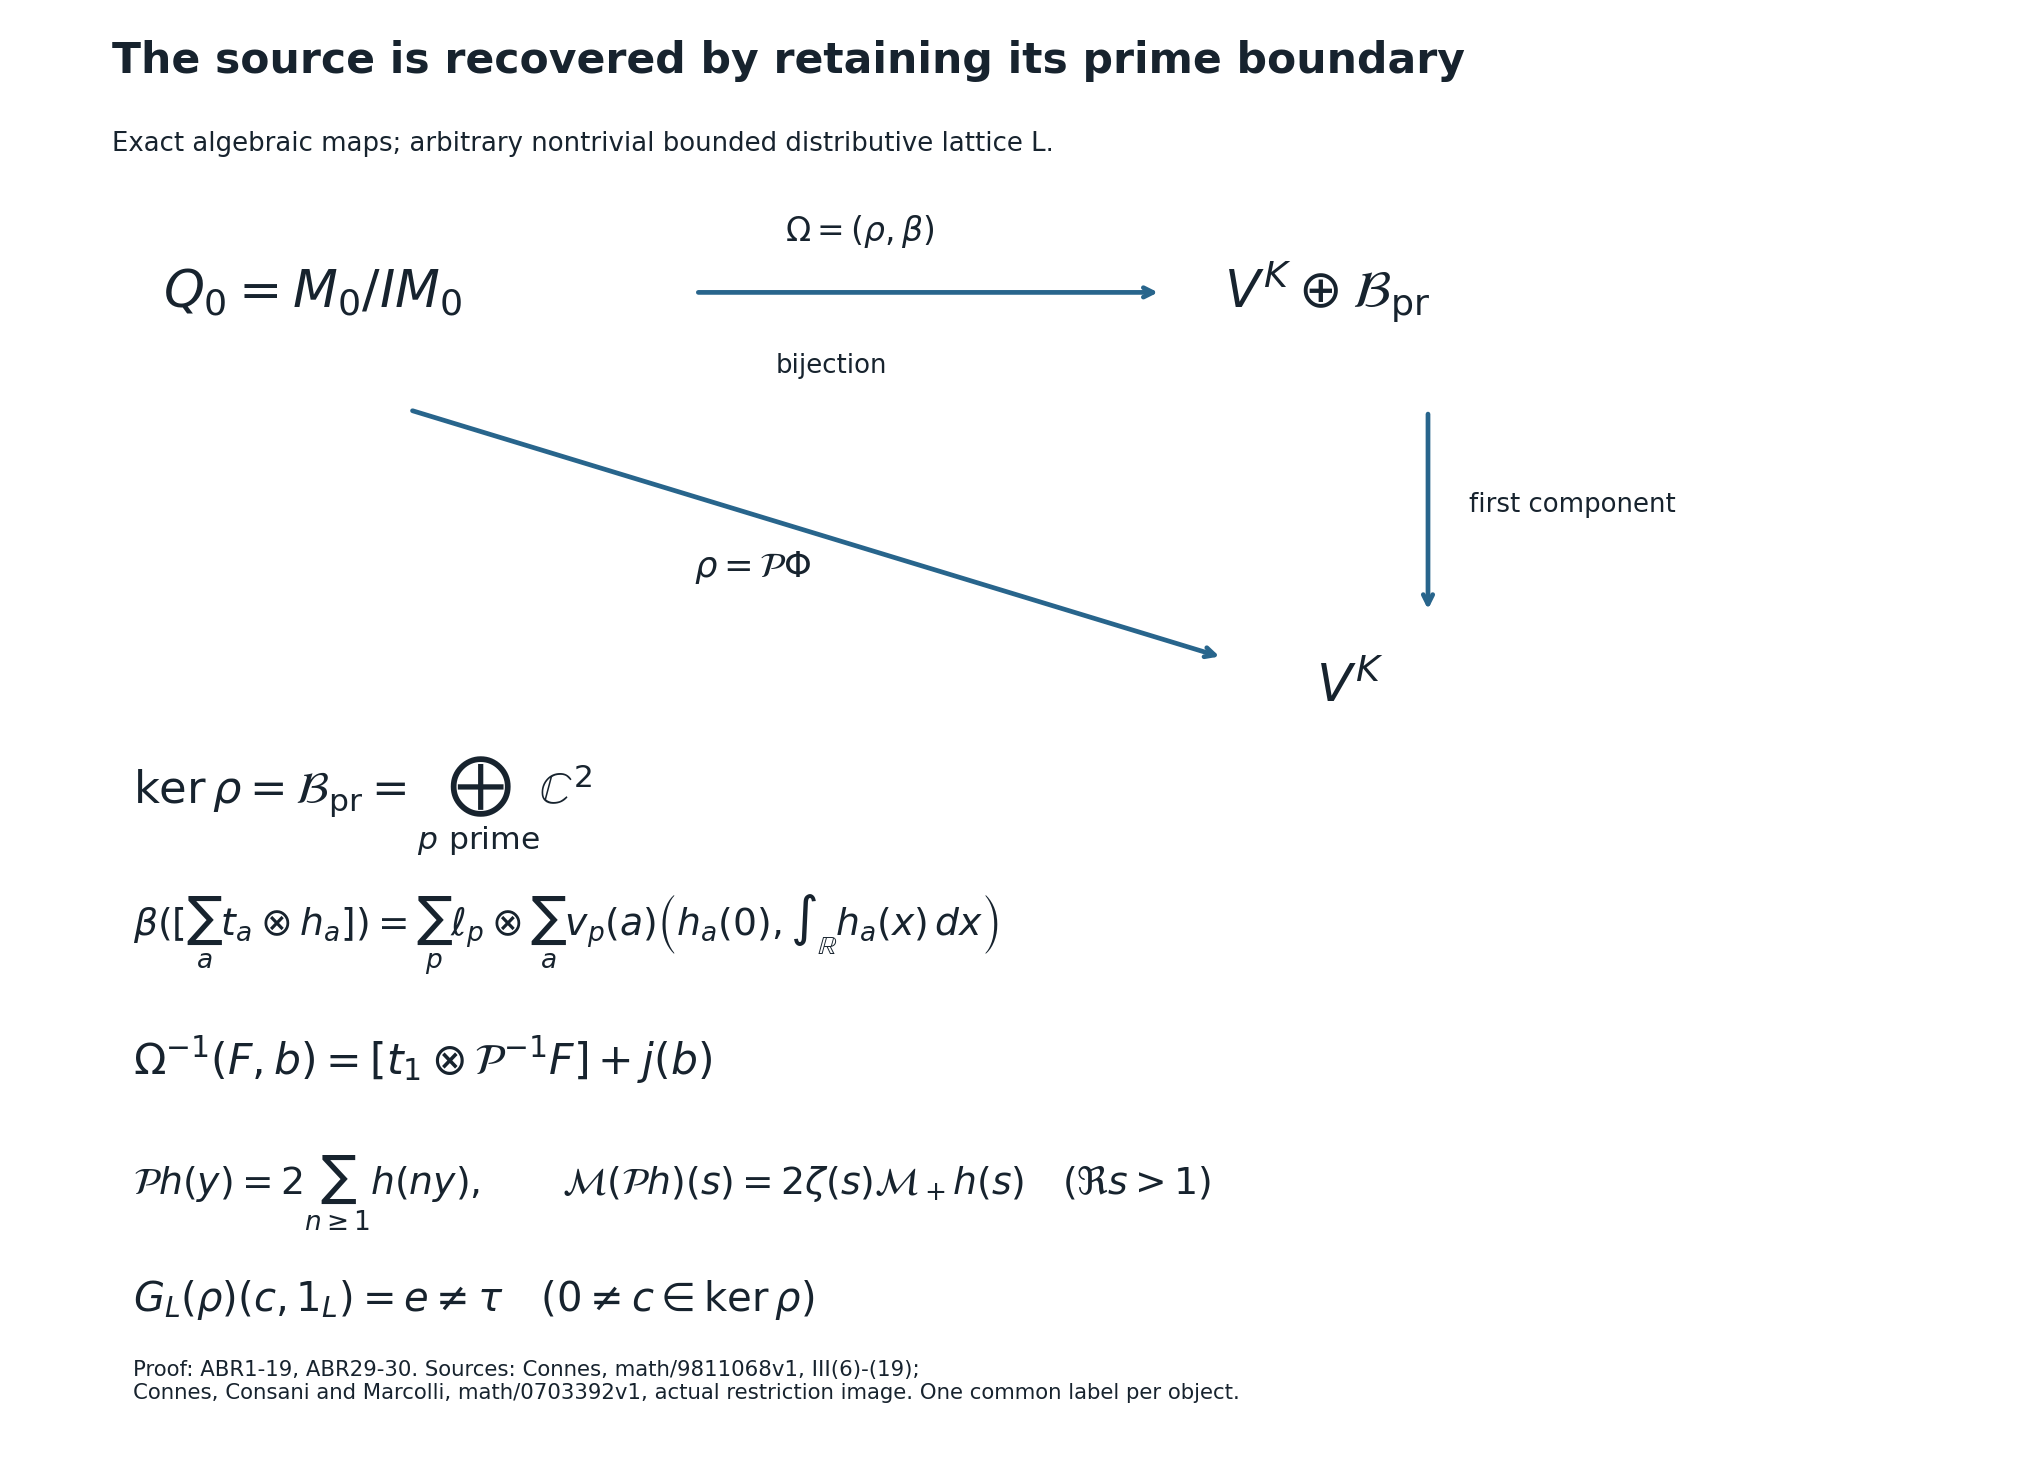
\includegraphics[width=\textwidth]{EXACT_SOURCE_RECOVERY.png}
\caption{The joint map retains all algebraic source information.
Periodization alone loses exactly the displayed prime boundary.
The lifted zero image retains its support label.}\end{figure}\clearpage
\begin{figure}[p]\centering
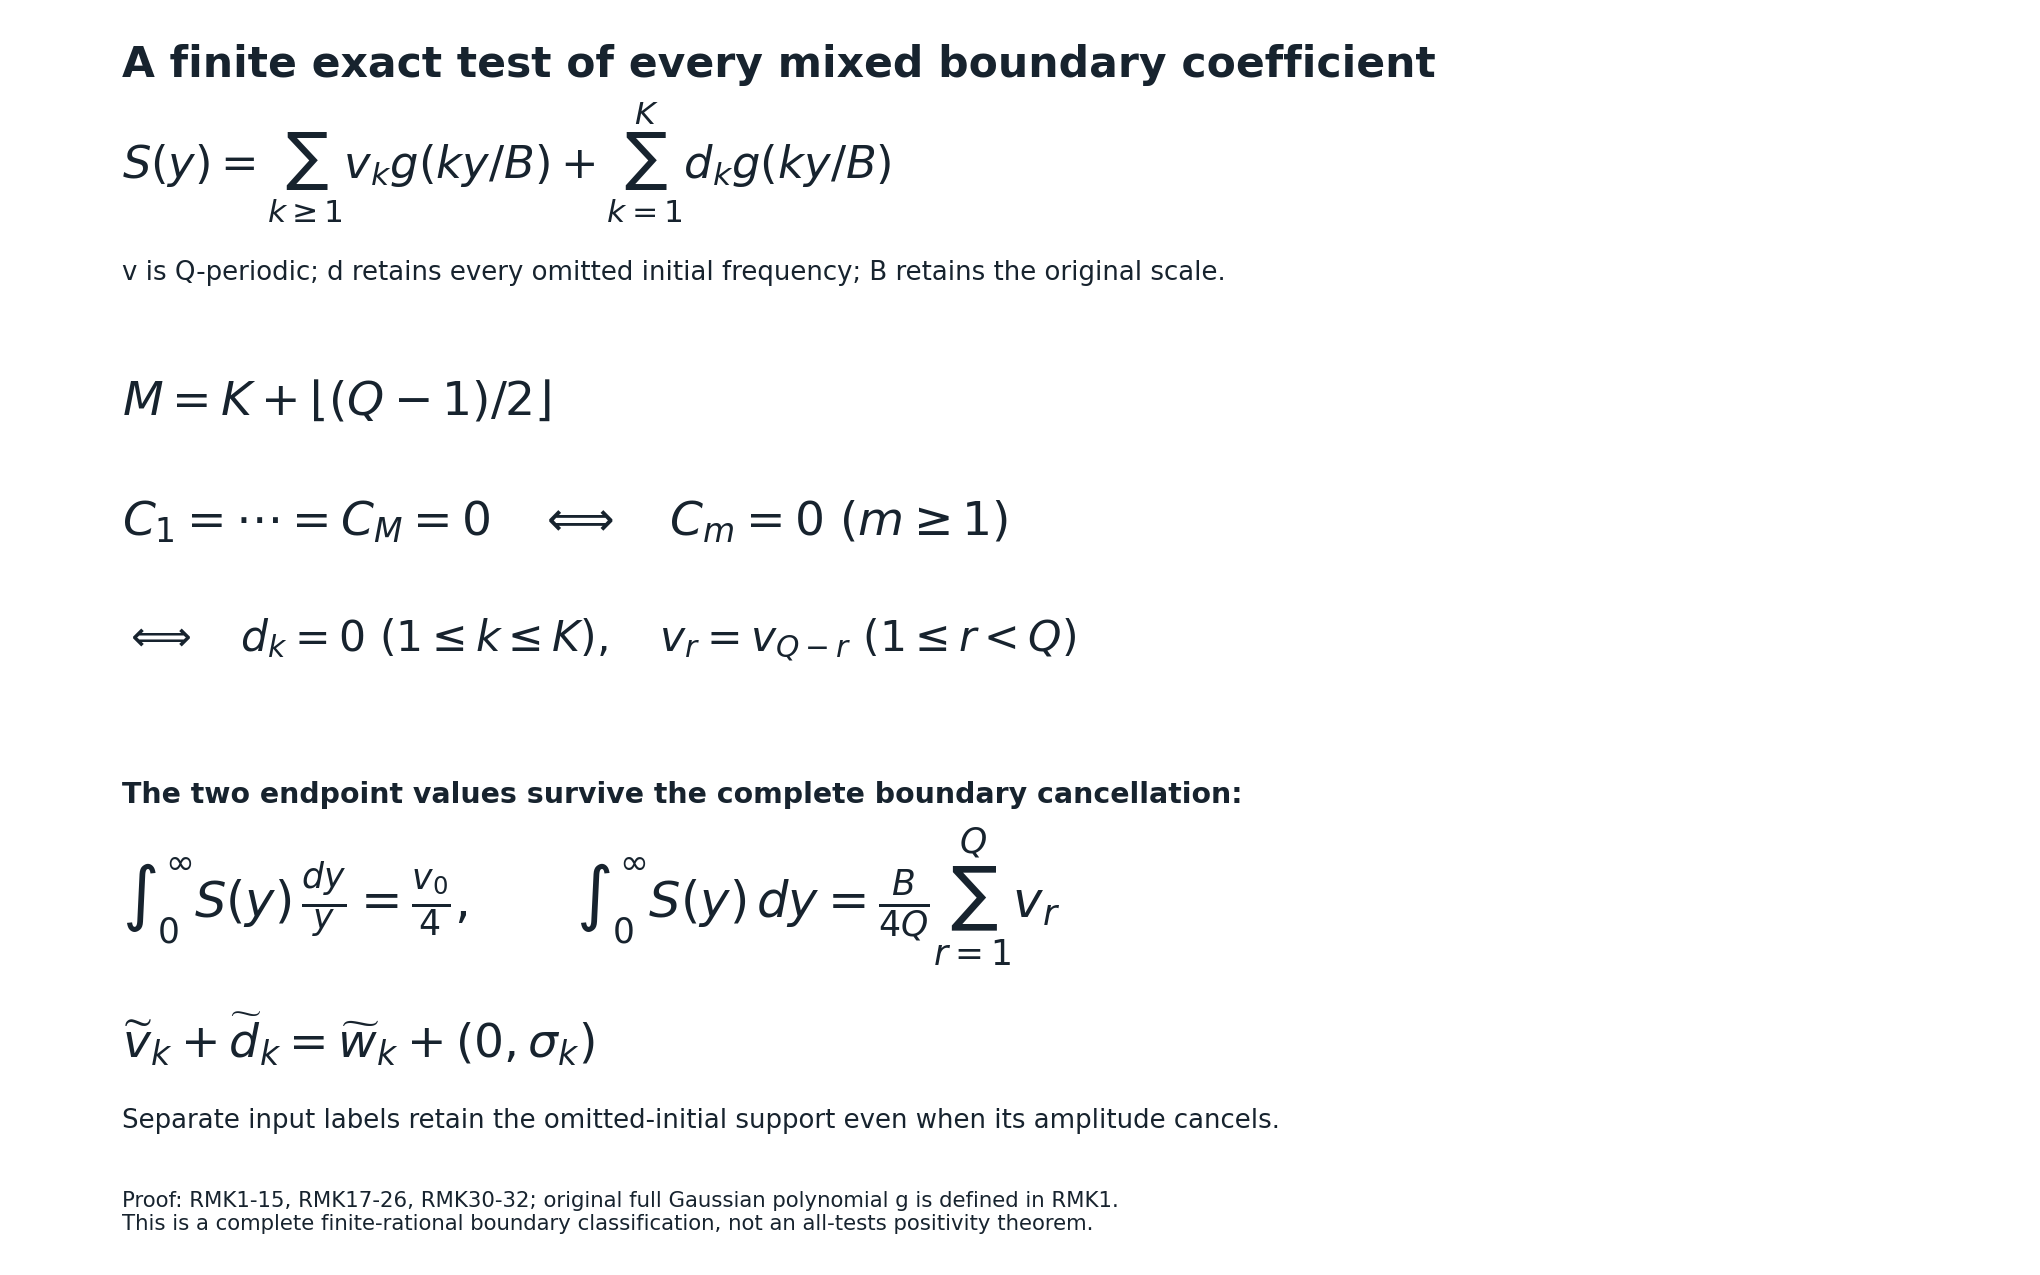
\includegraphics[width=\textwidth]{FINITE_MIXED_BOUNDARY.png}
\caption{A finite test determines the entire boundary in the stated
rational family. Its zero-boundary functions retain two distinct
endpoint values and their original support contributions.}\end{figure}
\clearpage

% Complete source: ORIGINAL_ZETA_THETA_CORRECTION.tex
% ZTC: original zeta, original shifted arithmetic family, retained theta data.
\section{Original zeta and the retained theta comparison}
\label{sec:original-zeta-theta-correction}

\paragraph{Correction and provenance.}
The statement that the Rodgers--Tao heat kernel was the programme's
original construction over the entire absolute base was not established.
THS1--31 begin with that classical analytic kernel and construct a
support-preserving coefficient lift. HTB1--35 establish its exact
comparison with the shifted Hurwitz family. Neither construction is a
derivation of the scalar kernel from the entire arithmetic geometry.
The distinction is measurable: THS22 already proves that all supported
zero times act identically on the actual theta orbit. The ambient
coefficient injection does not make that orbit injective.

The original arithmetic functions in this calculation remain
\begin{equation}\tag{ZTC1}
 \zeta(s)=\sum_{n=1}^{\infty}n^{-s},\qquad
 F_t(s)=\sum_{n=0}^{\infty}(n+1+t)^{-s},
 \qquad \operatorname{Re}s>1,\quad t>-1.
\end{equation}
Their continuations, endpoints, and exact shift generator are proved in
HTB2--5, with the programme source identified there by version, hash,
and original theorem labels. In particular $F_0=\zeta$,
$F_1=\zeta-1$, and $\partial_tF_t(s)=-sF_t(s+1)$.
The latter family comes from the supplied April 2026 shifted-Hurwitz
programme draft, not from a proposed identification of two time variables.
Brad Rodgers and Terence Tao's
\href{https://arxiv.org/abs/1801.05914v5}{original author source},
equations \texttt{phidef}, \texttt{htdef}, \texttt{hoz}, and
\texttt{sas}, supplies the auxiliary heat kernel used in THS and HTB.
These are cited inputs, not new discoveries. The following comparisons
are derived explicitly. Their complete HTB, THS, and CFD proofs accompany
this chapter.

\subsection{A direct theta sum for the original arithmetic family}

For real $t>-1$ and $x>0$, retain the actual shifted frequencies and put
\begin{equation}\tag{ZTC2}
 K_t(x)=\sum_{n=0}^{\infty}
               e^{-\pi(n+1+t)^2x}.
\end{equation}
This is a scalar analytic representation of the stated arithmetic
family. No assertion that it determines the full support lattice is
part of this definition. For fixed $a=1+t>0$, monotonicity of the
summand as a function of $n$ gives
\begin{equation}\tag{ZTC3}
 K_t(x)\le e^{-\pi a^2x}
              +\int_0^\infty e^{-\pi(a+y)^2x}\,dy
 \le 1+\frac1{2\sqrt x}.
\end{equation}
For $x\ge1$ the same bound after retaining the first exponential
gives $K_t(x)\le C_a e^{-\pi a^2x}$, since
$(a+n)^2-a^2\ge n^2$ and
$C_a=\sum_{n\ge0}e^{-\pi((a+n)^2-a^2)}<\infty$.
Consequently the following integral converges absolutely for
$\operatorname{Re}s>1$:
\begin{equation}\tag{ZTC4}
 \int_0^\infty x^{s/2-1}K_t(x)\,dx
   =\pi^{-s/2}\Gamma(s/2)F_t(s),\qquad
 F_t(s)=\frac{\pi^{s/2}}{\Gamma(s/2)}
                \int_0^\infty x^{s/2-1}K_t(x)\,dx.
\end{equation}
Indeed, with $\sigma=\operatorname{Re}s>1$, the sum of the
absolute termwise integrals equals
$\pi^{-\sigma/2}\Gamma(\sigma/2)\sum_{n\ge0}(n+a)^{-\sigma}$.
Fubini therefore applies. Substitution $y=\pi(n+a)^2x$ in each
term proves the displayed identity with its full Gamma and pi factors.
Continuation outside that domain means the meromorphic continuation
proved in HTB4, not an assertion that the unsubtracted integral converges
there.

There is also an exact inverse recovering the kernel, not only the
arithmetic function. For every real $c>1$,
\begin{equation}\tag{ZTC4a}
 K_t(x)=\frac1{4\pi i}\int_{c-i\infty}^{c+i\infty}
       \pi^{-s/2}\Gamma(s/2)F_t(s)x^{-s/2}\,ds.
\end{equation}
Here the integral is absolutely convergent. To prove the inversion
with its constant, set $\sigma=c/2>0$ and
$g(v)=\exp(\sigma v-e^v)$. This function and all its derivatives
are integrable on $\mathbb R$: at $-\infty$ they are bounded
by a constant times $e^{\sigma v}$, and at $+\infty$ by a
polynomial in $e^v$ times $g(v)$. The substitution $u=e^v$
identifies its Fourier transform with $\Gamma(\sigma-i y)$.
Repeated integration by parts therefore bounds that Gamma factor
by $C_N(1+|y|)^{-N}$ for every fixed $N$.
Fourier inversion gives
$e^{-u}=(2\pi i)^{-1}\int_{\sigma-i\infty}^{\sigma+i\infty}
\Gamma(w)u^{-w}\,dw$. One may verify this inversion directly
by first multiplying the Fourier integrand by $e^{-\epsilon y^2}$:
the resulting expression is the convolution of $g$ with the
Gaussian approximate identity, which converges to $g$; the stated
integrable transform bound permits dominated convergence as
$\epsilon\downarrow0$. Apply the identity to
$u=\pi(n+1+t)^2x$, then put $s=2w$. The resulting factor is
$1/(4\pi i)$. Finally sum in $n$. Interchange is justified by
$\sum(n+1+t)^{-c}<\infty$ and the integrable Gamma bound.
This proves ZTC4a. ZTC4 and ZTC4a are mutual recovery formulas
for the specified original arithmetic family and its scalar
theta sums; they do not recover a support lattice from a scalar
function.

Differentiation in $t$ is locally uniform for $t$ in compact subsets
of $(-1,\infty)$ and $x$ in compact subsets of $(0,\infty)$, by
Gaussian majorants for a polynomial times $e^{-c n^2}$.
It gives the exact formula
\begin{equation}\tag{ZTC5}
 \partial_tK_t(x)=-2\pi x\sum_{n=0}^{\infty}
              (n+1+t)e^{-\pi(n+1+t)^2x}.
\end{equation}
For $\operatorname{Re}s>0$, integration of its absolute value is
bounded by a constant times $\sum(n+a)^{-\sigma-1}$, locally
uniformly in $t$. More precisely its Mellin transform is
\begin{equation}\tag{ZTC6}
 \int_0^\infty x^{s/2-1}\partial_tK_t(x)\,dx
 =-2\pi^{-s/2}\Gamma(s/2+1)F_t(s+1)
 =-s\pi^{-s/2}\Gamma(s/2)F_t(s+1).
\end{equation}
Thus the original arithmetic shift generator is represented directly,
without substituting the heat generator for it. The stated equality
extends meromorphically by HTB4--5.

The separated sheet and its entire missing summand are visible before
any transform:
\begin{equation}\tag{ZTC7}
 K_1(x)=K_0(x)-e^{-\pi x},\qquad
 D_t(s)=\zeta(s)-F_t(s),\qquad D_1(s)=1,
\end{equation}
\begin{equation}\tag{ZTC8}
 \pi^{-s/2}\Gamma(s/2)D_t(s)
   =\int_0^\infty x^{s/2-1}\bigl(K_0(x)-K_t(x)\bigr)\,dx
       \quad(\operatorname{Re}s>1).
\end{equation}
ZTC7 follows by deleting the $n=1$ summand of $K_0$; ZTC8 follows
by subtracting two absolutely convergent integrals. At $t=1$ the
integral is exactly $\pi^{-s/2}\Gamma(s/2)$, so its inverse returns
the actual constant $1$, including its amplitude and support when lifted.

\subsection{Original zeta with both Mellin endpoints retained}

At $t=0$, HTB6 proves
\begin{equation}\tag{ZTC9}
 K_0(x)=x^{-1/2}K_0(1/x)+\tfrac12x^{-1/2}-\tfrac12.
\end{equation}
Split ZTC4 at $x=1$, apply this identity only to the integral over
$(0,1)$, and substitute $y=1/x$ there. Initially
$\operatorname{Re}s>1$, and direct integration gives
\begin{equation}\tag{ZTC10}
 \zeta(s)=\frac{\pi^{s/2}}{\Gamma(s/2)}
 \left\{
 \frac1{s-1}-\frac1s
 +\int_1^\infty K_0(x)
             \left(x^{s/2-1}+x^{-(s+1)/2}\right)\,dx
 \right\}.
\end{equation}
The two separate rational terms are the transforms of the two separate
terms $x^{-1/2}/2$ and $-1/2$. The integral on $[1,\infty)$ is
entire in $s$, since exponential decay bounds every logarithmic
derivative on compact subsets of the $s$-plane. This proves the
meromorphic continuation of the identity and keeps both endpoint
contributions. Neither has been declared zero or absorbed into an
unrecorded constant.

For the original cosine heat kernel, retain
\begin{equation}\tag{ZTC11}
\begin{gathered}
 A(s)=\frac{s(s-1)}2\pi^{-s/2}\Gamma(s/2),\qquad
 s(z)=\frac12+\frac{iz}{2},\qquad z(s)=-2i(s-1/2),\\
 H_0(z)=\frac{s(z)(s(z)-1)}{16}
           \pi^{-s(z)/2}\Gamma(s(z)/2)\zeta(s(z)),\\
 \zeta(s)=\frac{16\pi^{s/2}}
                  {s(s-1)\Gamma(s/2)}H_0(z(s)).
\end{gathered}
\end{equation}
The proof is HTB6--10: the exact Mellin substitution and two
integrations by parts yield the displayed multiplier, with all
endpoint limits justified in the original convergence half-plane.
The last equality is an identity of meromorphic functions. It is
not a licence to replace the original zeta calculation by an entire
function calculation while dropping its multiplier.

\subsection{The boundary is part of the receiving object}

Let $\mathcal M_s$ and $\mathcal M_z$ be the complex vector spaces
of meromorphic functions on the respective complex planes. Retain
the linear isomorphism, already proved in HTB11,
\begin{equation}\tag{ZTC12}
 Uf(z)=\frac{A(s(z))}{8}f(s(z)),\qquad
 U^{-1}G(s)=\frac{8G(z(s))}{A(s)}.
\end{equation}
Define the joint map on the entire two-component space by
\begin{equation}\tag{ZTC13}
 \mathcal V:\mathcal M_s\oplus\mathcal M_s
          \longrightarrow\mathcal M_z\oplus\mathcal M_z,
 \qquad (F,D)\longmapsto\bigl(U(F+D),UD\bigr).
\end{equation}
It has the exact inverse
\begin{equation}\tag{ZTC14}
 \mathcal V^{-1}(H,J)
    =\left(\frac{8(H-J)\circ z}{A},\frac{8J\circ z}{A}\right).
\end{equation}
Substitution proves both compositions equal the identity; all entries
are meromorphic functions, so no undefined product of separate
singular point values is involved. On the actual arithmetic family,
\begin{equation}\tag{ZTC15}
\begin{gathered}
 J_t=UD_t,\qquad
 \mathcal V(F_t,D_t)=(H_0,J_t),\\
 F_t(s)=\frac{16\pi^{s/2}}
              {s(s-1)\Gamma(s/2)}
              \bigl(H_0(z(s))-J_t(z(s))\bigr),\\
 J_1(z)=\frac{A(s(z))}{8},\qquad
 J_t(i)=-\frac t8.
\end{gathered}
\end{equation}
For the last equality use HTB5:
$D_t(0)=\zeta(0)-F_t(0)=t$, $A(0)=-1$, and $z(0)=i$.
In particular the retained pair determines the real parameter $t$
by $t=-8J_t(i)$. All $t$ give the same first component $H_0$.
Discarding $J_t$ therefore identifies different actual arithmetic
inputs. This is an explicit failure of injectivity on the actual
programme family, not merely an example in an unrelated vector space.
On the unrestricted space the summation map $(G,J)\mapsto G+J$
has exactly the kernel $\{(B,-B):B\in\mathcal M_z\}$.

For the complete support carrier, use the common label on the
direct sum:
\begin{equation}\tag{ZTC16}
 G_L(\mathcal M_s\oplus\mathcal M_s)
   \xrightarrow{\mathcal V^\uparrow}
 G_L(\mathcal M_z\oplus\mathcal M_z),\qquad
 ((F,D),\lambda)\longmapsto(\mathcal V(F,D),\lambda).
\end{equation}
Here $G_L(V)=\{(0,\lambda):\lambda\in L\}\cup(V\times\{1_L\})$
with its original joins and meets. Additivity, compatibility with
the $G_L(\mathbb C)$ action, carrier membership, and the inverse
follow componentwise from linearity and ZTC14, as explicitly proved
in CFD11--12. This is a bijection for every bounded distributive $L$.
It does not silently replace the common label by independent labels
on two product factors. In particular $e=(0,1_L)$ and
$\tau=(0,0_L)$ remain distinct when $L$ is nontrivial.

\paragraph{The exact multiplication comparison.}
The preceding maps were declared as linear and semimodule maps.
Their injectivity does not identify the original multiplication with
ordinary multiplication of their images. This can be checked exactly,
without discarding the completion multiplier. Set
\begin{equation}\tag{ZTC16a}
 B(z)=\frac{A(s(z))}{8}
 =\frac{s(z)(s(z)-1)}{16}
       \pi^{-s(z)/2}\Gamma(s(z)/2).
\end{equation}
For meromorphic $f,g$ on the $s$-plane the two products are
\begin{equation}\tag{ZTC16b}
\begin{gathered}
 U(fg)(z)=B(z)f(s(z))g(s(z)),\\
 (Uf)(z)(Ug)(z)=B(z)^2f(s(z))g(s(z)).
\end{gathered}
\end{equation}
In particular $U1=B$, not the ordinary constant unit. The factor
$B$ is nonconstant: it has a zero at $z(1)=-i$ and poles at
$z(-2m)$, $m\ge1$. Thus ordinary multiplication is not preserved.
The exact transported product and its unit are
\begin{equation}\tag{ZTC16c}
 G\odot H=\frac{8G(z)H(z)}{A(s(z))},\qquad
 1_{\odot}(z)=\frac{A(s(z))}{8}.
\end{equation}
This formula is an identity of meromorphic functions, including
their germs at the zeros and poles of the multiplier. It is not
pointwise division of undefined singular values. Substitution
gives $(Uf)\odot(Ug)=U(fg)$. Directly,
$(G\odot H)\odot K=GHK/B^2=G\odot(H\odot K)$,
$B\odot G=G$, and distributivity follows from distributivity of
meromorphic multiplication. Together with ZTC12 this proves a
unital algebra isomorphism with the stated product.

For each local holomorphic ring $\mathcal O_{s_0}$ the affine
coordinate map identifies it with $\mathcal O_{z(s_0)}$.
Its exact image under $U$ is the embedded fractional lattice
$B\mathcal O_{z(s_0)}$. This lattice is closed under $\odot$,
since $(Bu)\odot(Bv)=Buv$, and has unit $B$.
Keeping instead the unmodified target $\mathcal O_{z(s_0)}$
can fail closure: at $s_0=1$, $B$ has a simple zero, so
$1\odot1=1/B$ is not holomorphic. This image-lattice statement
differs from the preimage lattice $A^{-1}\mathcal O$ in ZTC17:
the former transports an original holomorphic ring, whereas the
latter specifies which original meromorphic sections have a
holomorphic completed image.

The full support carrier admits the same exact comparison. Retain
its original addition, and define the target product by
\begin{equation}\tag{ZTC16d}
 (G,\lambda)\odot_L(H,\mu)
   =\left(\frac{8GH}{A\circ s},\lambda\wedge\mu\right),
 \qquad 1_{\odot_L}=(B,1_L).
\end{equation}
If the amplitude of a product is nonzero, both input amplitudes
are nonzero, hence both labels are $1_L$; this proves carrier
closure. If either amplitude is zero its output amplitude is
zero and the displayed meet retains its original label.
Associativity and distributivity follow from ZTC16c and the
meet/join laws of the bounded distributive lattice. The map
$(f,\lambda)\mapsto(Uf,\lambda)$ and its inverse therefore
give a unital semiring isomorphism from the original coefficient
semiring to this specified target, preserving $e$ and $\tau$.
An ideal $P$ is sent to its literal image $U^{\uparrow}(P)$;
closure under addition and multiplication follows by applying the
isomorphism. Its inverse proves the converse. Moreover a product
belongs to that image precisely when the corresponding original
product belongs to $P$, proving that prime ideals correspond.
This proves the exact spectrum comparison for these specified
coefficient semirings. It is not a derivation of the entire
arithmetic base from the scalar function $H_0$.

For ZTC13--16, no multiplication on pairs was specified: the
proved assertion there remains a common-label semimodule
isomorphism. Neither ordinary multiplication nor a Weil pairing
is silently inferred from that assertion.

\subsection{Local zeros, poles, and the original trace}

The earlier conversational assertion that the singular module map
had not been established was also too broad: HTB13 already proves
$A^{-1}\mathcal O\xrightarrow{U}\mathcal O$ with the affine
coordinate change. CFD1--10 now make the comparison with the
\emph{original} regular lattice and every finite jet explicit.
At a finite point let $h=s-s_0$ and $A=h^k a(h)$, $a(0)\ne0$.
Retain $I=A^{-1}\mathcal O=h^{-k}\mathcal O$ as an embedded
submodule of the meromorphic germs, and $J=I\cap\mathcal O$.
For nonzero $f\in I$ the original order is
\begin{equation}\tag{ZTC17}
 \operatorname{ord}_{s_0}f
 =\dim_{\mathbb C}(I/\mathcal O f)
  -\dim_{\mathbb C}(I/J)
  +\dim_{\mathbb C}(\mathcal O/J).
\end{equation}
This is proved by the power-of-$h$ bases in CFD6--7, without
identifying the reference lattices. At a trivial zero $s_0=-2m$,
$I=h\mathcal O$, $I/\mathcal O\zeta=0$ and
$\mathcal O/I$ has dimension $1$. At $s_0=1$,
$I=h^{-1}\mathcal O$, $I/\mathcal O\zeta=0$ and
$I/\mathcal O$ has dimension $1$. Their signs in ZTC17 give,
respectively, $+1$ and $-1$. At $s_0=0$, $A(0)=-1$ is a unit.
CFD4 provides the invertible triangular matrices recovering all
Laurent coefficients with the exact factors $8$ and $i/2$.
Keeping only the zero algebra of the completed section would give
zero in both cancelled cases; keeping these comparison modules
restores the actual divisor.

The earlier conversational explanation of the fibres requires a
further correction. The map
\begin{equation}\tag{ZTC17a}
 \mathcal O/h\mathcal O\longrightarrow
 h\mathcal O/h^2\mathcal O,\qquad [u]\longmapsto[hu]
\end{equation}
is an isomorphism of $\mathcal O$-modules. It is well-defined because
$h(h\mathcal O)=h^2\mathcal O$, surjective by the definition of
$h\mathcal O$, and injective because $hu\in h^2\mathcal O$ implies
$u\in h\mathcal O$ in the local integral domain. Its inverse is
$[hu]\mapsto[u]$. Consequently the two abstract fibres alone do
not account for the loss. What must be retained is their specified
embedding and the original reference lattice: multiplication by
$A=h^{-1}a(h)$ identifies $I=h\mathcal O$ with $\mathcal O$, but
the length-one quotient $\mathcal O/I$ records the cancelled
original zero. Replacing the entire marked comparison by the
completed section's zero quotient discards precisely that datum.
Likewise multiplication by nonzero meromorphic $A$ is an
automorphism of the meromorphic sheaf as a module. It is not
a ring automorphism for ordinary multiplication, as ZTC16b proves.
It is not an automorphism
of the fixed holomorphic lattice at its zeros and poles. These
category statements do not contradict one another.

Logarithmic differentiation gives the original trace identity
\begin{equation}\tag{ZTC18}
 \frac{\zeta'(s)}{\zeta(s)}
 =-2i\frac{H_0'(z(s))}{H_0(z(s))}
 -\frac1s-\frac1{s-1}+\frac12\log\pi-\frac12\psi(s/2).
\end{equation}
It first holds away from zeros and poles and then meromorphically;
$\psi=\Gamma'/\Gamma$. For a positively oriented finite contour
$\gamma$ avoiding all zeros and poles of the functions and all
singularities of every displayed integrand, and a holomorphic test $g$
on and inside it, multiplication by $g$ and integration gives
\begin{equation}\tag{ZTC19}
\begin{split}
 \frac1{2\pi i}\int_\gamma g\,\frac{\zeta'}\zeta\,ds
 ={}&\frac1{2\pi i}\int_\gamma
           g(s)(-2i)\frac{H_0'(z(s))}{H_0(z(s))}\,ds\\
 &-\frac1{2\pi i}\int_\gamma g(s)
   \left(\frac1s+\frac1{s-1}-\frac12\log\pi
                         +\frac12\psi(s/2)\right)ds.
\end{split}
\end{equation}
At every zero or pole, write a meromorphic function as
$(s-s_0)^r$ times a holomorphic unit. Its logarithmic derivative
then has residue $r$. The residue theorem proves that ZTC19
counts the original zeros with multiplicity and the original poles
with negative multiplicity, including every trivial zero inside
the contour. No infinite-contour limit or decay assumption is
hidden here. Extending this finite identity to a particular infinite
trace requires the actual convergence estimates of that trace.

\subsection{Two different trajectories through the same original zeta}

The original-$s$ function associated with the classical heat path is
\begin{equation}\tag{ZTC20}
 f_h^{\rm heat}(s)=\frac{16\pi^{s/2}}
                         {s(s-1)\Gamma(s/2)}H_h(z(s)),
 \qquad f_0^{\rm heat}=\zeta.
\end{equation}
CFD18--21 give its full receiving operator and prove
\begin{equation}\tag{ZTC21}
 \left.\partial_hf_h^{\rm heat}(-2)\right|_{h=0}=0,
 \qquad
 \left.\partial_tF_t(-2)\right|_{t=0}=-\frac16.
\end{equation}
For completeness, the heat equation and chain rule give
$\partial_hf=(Af)''/(4A)$. At $h=0$, $A\zeta$ is holomorphic
at $-2$ whereas $1/A$ has a simple zero there, giving the first
value. HTB5 gives the second as $2\zeta(-1)=-1/6$.
The discrepancy holds on the actual initial arithmetic function.
CFD21 further proves that all the zeros at $-2m$ remain simple
along the real heat path, while its residue at $1$ varies strictly;
the actual Hurwitz path has constant residue $1$ and values
$-B_{2m+1}(1+t)/(2m+1)$ at those points.

Thus the valid original-$\zeta$ receiver consists of the original
functions, their exact transform and inverse, the retained boundary
component, the embedded local comparison modules, and all support
labels. The scalar theta orbit by itself is a smaller observable.
These proofs neither exhibit an off-line zero of the original
$\zeta$ nor rule one out. They establish precisely which input and
which deformation a subsequent estimate is estimating.

\clearpage

% Complete source: CC_ADELIC_COINVARIANT_BRIDGE_INDEPENDENT.tex
% Independent derivation for the root's actual-adelic/coinvariant bridge.
% Algebraic quotients only; no assertion about an unproved topological quotient.
\section{The actual adelic source and its retained prime boundary}
\label{sec:independent-adelic-coinvariant-bridge}

The adelic restriction operation and its original measures are those of
Alain Connes, \emph{Trace formula in noncommutative geometry and the zeros
of the Riemann zeta function},
\href{https://arxiv.org/abs/math/9811068v1}{Section III (6)--(19)},
and Alain Connes, Caterina Consani and Matilde Marcolli,
\href{https://arxiv.org/abs/math/0703392v1}{\emph{The Weil proof and the
geometry of the adeles class space}}, as specified in SWQ2--14.
The homological complex used below is the standard Koszul complex,
named for Jean-Louis Koszul. The standard regular-sequence mechanism is
recorded by \emph{The Stacks Project Authors},
\href{https://stacks.math.columbia.edu/tag/062F}{Tag 062F}, with
\href{https://github.com/stacks/stacks-project/blob/a04446e57ec1fbc252a871afcec7752fb2807b14/more-algebra.tex#L7264}{original
author TeX, lines 7264--7298, commit
\texttt{a04446e57ec1fbc252a871afcec7752fb2807b14}}.
The contribution here is the exact application, connecting representatives,
and receiving maps for these specified programme modules; the necessary
Koszul exactness is proved below as well. All tensor products and
quotients below are algebraic unless a different meaning is explicitly
stated.

The precise public programme inputs are
\href{https://github.com/KokunoYumeto/zeta-function-research-reader/blob/acd7016b8232a56f31ae3e69fb800571e8789080/workbenches/splitzero-tandem/continuations/20260923-retained-source-readers/original-zeta-full-boundary/CC_WEIL_BOUNDARY_READER.tex#L927}{SWQ2--14},
\href{https://github.com/KokunoYumeto/zeta-function-research-reader/blob/acd7016b8232a56f31ae3e69fb800571e8789080/workbenches/splitzero-tandem/continuations/20260923-retained-source-readers/original-zeta-full-support/MASS_THETA_PRIME_RECEIVER.tex#L12}{MRT1--20}, and
\href{https://github.com/KokunoYumeto/zeta-function-research-reader/blob/acd7016b8232a56f31ae3e69fb800571e8789080/workbenches/splitzero-tandem/continuations/20260923-retained-source-readers/endpoint-resonance/ENDPOINT_RESONANCE_AND_PRIME_CLASS.tex#L430}{ER27--30}.
These pinned proof targets were checked against the local source versions.

\subsection{The finite adelic basis and the exact original source}

Put
\begin{equation}\tag{ABR1}
 G=\mathbb Q_{>0}^{\times},\quad R=\mathbb C[G],\quad
 I=\ker(\varepsilon:R\longrightarrow\mathbb C),\quad
 H=\mathcal S_{\rm even}(\mathbb R),\quad
 K=\widehat{\mathbb Z}^{\times},\quad c_a=1_{a\widehat{\mathbb Z}}.
\end{equation}
The basis element $t_a\in R$ satisfies $t_at_b=t_{ab}$ and
$\varepsilon(t_a)=1$. The finite additive measure has
$\operatorname{vol}(\mathbb Z_p)=1$, and the real additive measure
is Lebesgue measure. Thus
\begin{equation}\tag{ABR2}
 \operatorname{vol}(a\widehat{\mathbb Z})
  =\prod_p p^{-v_p(a)}=a^{-1}\qquad(a>0\text{ rational}).
\end{equation}
This equality uses the original positive real value of $a$ and its
prime factorization; the finite and real factors will both be retained.

The family $(c_a)_{a\in G}$ is a vector-space basis of
$\mathcal S(\mathbb A_f)^K$. To prove spanning, first observe that a
compactly supported locally constant function on $\mathbb Q_p$,
invariant under $\mathbb Z_p^\times$, is constant on valuation shells.
Choose integers $A\le B$ such that its support is in $p^A\mathbb Z_p$
and it is constant on cosets of $p^B\mathbb Z_p$. If its values on
the shells $A\le n<B$ and on the last ball $p^B\mathbb Z_p$ are
$d_A,\ldots,d_B$, the function is exactly
\[
 d_A1_{p^A\mathbb Z_p}
 +\sum_{n=A+1}^{B}(d_n-d_{n-1})1_{p^n\mathbb Z_p}.
\]
The original Bruhat space on $\mathbb A_f$ consists of finite sums
of restricted tensor products with $1_{\mathbb Z_p}$ outside a finite
set of primes. Compact-unit averaging of a finite-place test is a
finite linear operation: its support is contained in finitely many
bounded local balls and its local-constancy subgroups have finite
index there. Averaging therefore reduces to a finite quotient. Apply
the preceding local formula at the finitely many relevant primes and
expand the finite tensor products. Their balls are exactly $c_a$.
For an invariant test averaging leaves the test itself fixed, which
proves spanning.

For independence, take distinct $a_1,\ldots,a_m\in G$ and partially
order them by $a_i\preceq a_j$ when $a_j/a_i$ is an integer. This is
a partial order because both positive ratios can be integers only
when they are one. Order this finite set by a linear extension.
Evaluate its characteristic functions at the finite rational ideles
$x_f=a_j$. Then
\[
 c_{a_i}(a_j)=1\quad\Longleftrightarrow\quad a_i\preceq a_j.
\]
Indeed $\mathbb Q\cap\widehat{\mathbb Z}=\mathbb Z$.
The resulting matrix is lower triangular with diagonal one. Its
determinant is one, proving independence. This proof also works for
coefficients in any complex vector space, because back substitution
uses only this finite triangular matrix.

Define
\begin{equation}\tag{ABR3}
 \Theta:R\otimes H\longrightarrow
           \mathcal S(\mathbb A_{\mathbb Q})^{K,\mathrm{even}},
 \qquad
 \Theta(t_a\otimes h)(x_\infty,x_f)
       =h(x_\infty/a)c_a(x_f).
\end{equation}
Here evenness refers to the original real variable $x_\infty$.
Every target is a finite sum $\sum_a g_a(x_\infty)c_a(x_f)$ with
$g_a\in H$. Set $h_a(x)=g_a(ax)$ to obtain its preimage in ABR3.
Independence follows from the vector-valued independence of the
$c_a$ and the injectivity of each real dilation. Thus $\Theta$ is
an isomorphism of vector spaces, with the displayed exact inverse.
No change in the original real coordinate has been made in the target.

For $r\in G$ define full rational adelic dilation by
$\alpha_r\xi(x)=\xi(r^{-1}x)$. The finite argument gives
$c_a(r^{-1}x_f)=c_{ra}(x_f)$, while the real argument is
$h(x_\infty/(ra))$. Consequently
\begin{equation}\tag{ABR4}
 \alpha_r\Theta(t_a\otimes h)=\Theta(t_{ra}\otimes h).
\end{equation}
This is the left $R$-action. It is full diagonal rational dilation;
it is not dilation of the real idele-class coordinate alone.

Let $m(h)=(h(0),\int_{\mathbb R}h(x)\,dx)$. Evaluation and
integration of ABR3 give the two exact moments
\begin{equation}\tag{ABR5}
 \Theta(t_a\otimes h)(0)=h(0),\qquad
 \int_{\mathbb A}\Theta(t_a\otimes h)
     =a\left(\int_{\mathbb R}h\right)
                     \prod_p p^{-v_p(a)}=\int_{\mathbb R}h.
\end{equation}
Thus $(\varepsilon_0,\varepsilon_1)\Theta=\varepsilon\otimes m$.
In particular
\begin{equation}\tag{ABR6}
 M_0=\ker(\varepsilon\otimes m),\qquad H_{00}=\ker m,
 \qquad
 \Theta(M_0)=\mathcal S(\mathbb A)_0^{K,\mathrm{even}}.
\end{equation}
This is equality of the actual spaces with their two original
endpoint conditions, not a comparison only after completion.

\subsection{The complete algebraic coinvariant and its boundary}

The two even Schwartz functions
\[
 h_0(x)=(1-2\pi x^2)e^{-\pi x^2},\qquad
 h_1(x)=2\pi x^2e^{-\pi x^2}
\]
have moments $(1,0)$ and $(0,1)$. Indeed their evaluations are
immediate and the real Gaussian integrals are
$\int e^{-\pi x^2}=1$ and $\int x^2e^{-\pi x^2}=1/(2\pi)$.
The section $\sigma(u_0,u_1)=u_0h_0+u_1h_1$ therefore splits $m$.
It gives
\begin{equation}\tag{ABR7}
 M_0=(R\otimes H_{00})\oplus(I\otimes\sigma(\mathbb C^2)),
 \qquad
 Q_0=M_0/IM_0\cong H_{00}\oplus(I/I^2)\otimes\mathbb C^2.
\end{equation}
Indeed multiplication by $I$ has exactly the two components
$I\otimes H_{00}$ and $I^2\otimes\sigma(\mathbb C^2)$.

For clarity the resulting boundary and inverse can be written
without leaving a dependence on the chosen moment section. Put
\begin{equation}\tag{ABR8}
 W=\bigoplus_{p\ \mathrm{prime}}\mathbb C\ell_p,
 \qquad \mathcal B_{\mathrm{pr}}=W\otimes\mathbb C^2.
\end{equation}
The map $[t_a-1]\mapsto\sum_pv_p(a)\ell_p$ is an isomorphism
$I/I^2\to W$. For its proof retain the identity
$t_{ab}-1=(t_a-1)+(t_b-1)+(t_a-1)(t_b-1)$.
Modulo $I^2$ it gives additivity, and inversion gives the negative
of a class. Prime factorization expresses each class as the stated
sum. For independence the functionals
$D_p(\sum_ac_at_a)=\sum_ac_av_p(a)$ satisfy
$D_p(rs)=\varepsilon(r)D_p(s)+\varepsilon(s)D_p(r)$, and hence
vanish on $I^2$. They take value one on $[t_p-1]$ and zero on
the other displayed prime generators.

The canonical coordinates of $c=[\sum_at_a\otimes h_a]\in Q_0$
are
\begin{equation}\tag{ABR9}
 \Phi(c)=\sum_a h_a\in H_{00},\qquad
 \beta(c)=\sum_p\ell_p\otimes\sum_a v_p(a)m(h_a).
\end{equation}
Both maps kill $IM_0$. For $\beta$, apply the preceding derivation
identity to a product $r\sum_at_a\otimes h_a$, $r\in I$;
its value is $\sum_pD_p(r)\ell_p\otimes\sum_am(h_a)=0$ by
the defining moment condition. The inverse of ABR9 sends
\begin{equation}\tag{ABR10}
 (h,\sum_p\ell_p\otimes u_p)
 \longmapsto [t_1\otimes h]
             +\sum_p[(t_p-1)\otimes\sigma(u_p)].
\end{equation}
Only finitely many $u_p$ are nonzero. Changing $\sigma$ changes
the latter expression by an element of $I\otimes H_{00}\subset IM_0$.
To check the inverse on an arbitrary representative, subtract
$t_1\otimes\sum_a h_a$ and write the remainder as
$\sum_a(t_a-1)\otimes h_a$. Replacing each $h_a$ there by
$\sigma m(h_a)$ changes its class by $IM_0$, and ABR8 then
gives exactly ABR10. Thus the short exact sequence
\begin{equation}\tag{ABR11}
 0\longrightarrow\mathcal B_{\mathrm{pr}}
   \xrightarrow{\ j\ }Q_0\xrightarrow{\Phi}H_{00}
   \longrightarrow0
\end{equation}
is canonically split by $h\mapsto[t_1\otimes h]$, and $j$ is
the section-independent second term of ABR10.

\subsection{Actual periodization, injectivity, and exact inverse}

For the original restriction map
$E\xi(u,y)=\sum_{q\in\mathbb Q^\times}\xi(qy,qu)$,
$u\in K$, $y>0$, the finite condition in ABR3 is
$q/a\in\widehat{\mathbb Z}\cap\mathbb Q=\mathbb Z$.
Hence $q=an$ for $n\in\mathbb Z\setminus\{0\}$. It follows that
\begin{equation}\tag{ABR12}
 E\Theta(t_a\otimes h)(u,y)
    =\sum_{n\in\mathbb Z\setminus\{0\}}h(ny)
    =2\sum_{n\ge1}h(ny)=:\mathcal P h(y).
\end{equation}
Evenness of $h$ supplies exactly the last factor two. The real
and finite scales $a$ have both participated in the equality;
no finite restriction has been dropped. All sums are locally
absolutely convergent with every real derivative by Schwartz decay.
For $m=\sum_at_a\otimes h_a\in M_0$, ABR12 is
$E\Theta(m)=\mathcal P(\sum_a h_a)$.

The Fourier convention
$\widehat h(\xi)=\int_{\mathbb R}h(x)e^{-2\pi ix\xi}\,dx$
gives the exact Poisson identity with both endpoints
\begin{equation}\tag{ABR13}
 \mathcal P h(y)
 =y^{-1}\mathcal P\widehat h(1/y)
     +y^{-1}\int_{\mathbb R}h(x)\,dx-h(0).
\end{equation}
For $h\in H_{00}$ both displayed endpoint terms are zero, and
$\widehat h$ also belongs to $H_{00}$ because
$\widehat h(0)=\int h=0$ and $\int\widehat h=h(0)=0$.
At infinity the sums of every Euler derivative of $\mathcal P h$
decay faster than every power: choose an arbitrarily large Schwartz
power $A>1$ and bound their sums by a constant times
$y^{-A}\sum n^{-A}$. ABR13 proves the corresponding estimates
at zero. Therefore $\mathcal P h$ belongs to the original radial
strong Schwartz test space. All powers of $\log y$ are also
controlled by these bounds, so its Mellin transform is entire.

For $\Re s>1$, absolute Fubini gives the original identity
\begin{equation}\tag{ABR14}
 \mathcal M(\mathcal P h)(s)
   =2\zeta(s)\mathcal M_+h(s),\qquad
 \mathcal M_+h(s)=\int_0^\infty h(x)x^{s-1}\,dx.
\end{equation}
Indeed the absolute sum of integrals is
$2\zeta(\Re s)\int_0^\infty|h(x)|x^{\Re s-1}\,dx<\infty$.
The original Euler product proves that $\zeta(s)\ne0$ in this
half-plane: the logarithms of its factors converge absolutely
because $\sum_p\sum_{k\ge1}p^{-k\Re s}/k<\infty$.
Thus division by the actual $2\zeta(s)$ is valid on the exact
domain used below. There is no completed replacement of $\zeta$.

For $\sigma>1$, $g_\sigma(v)=e^{\sigma v}h(e^v)$ is Schwartz
on $\mathbb R$. Every derivative is a finite sum of
$e^{(\sigma+j)v}h^{(j)}(e^v)$. These decay exponentially at
$-\infty$ and faster than any prescribed exponential at
$+\infty$, using the original real Schwartz estimates.
Consequently $\mathcal M_+h(\sigma+it)$ decays faster than
every power of $t$. Fourier inversion in $v$ gives
\begin{equation}\tag{ABR15}
 h(x)=\frac1{4\pi i}
   \int_{\sigma-i\infty}^{\sigma+i\infty}
      \frac{\mathcal M(\mathcal P h)(s)}{\zeta(s)}x^{-s}\,ds,
       \qquad x>0,\quad\sigma>1.
\end{equation}
Every constant is explicit: Mellin inversion has $1/(2\pi i)$,
and ABR14 contributes the additional $1/2$. To justify inversion
directly, multiply the Fourier integrand by $e^{-\epsilon t^2}$.
Its inverse is convolution with
$(4\pi\epsilon)^{-1/2}e^{-v^2/(4\epsilon)}$, which tends to
$g_\sigma$ as $\epsilon\downarrow0$. The proved rapid vertical
decay permits dominated convergence on the Fourier side. This
proves ABR15, including absolute convergence. Evenness recovers
$h(x)$ for $x<0$ and $h(0)=0$ supplies the remaining point.
In particular $\mathcal P$ is injective on $H_{00}$.

There is also an exact arithmetic inverse in the original variable:
\begin{equation}\tag{ABR15a}
 h(x)=\frac12\sum_{n\ge1}\mu(n)\mathcal P h(nx),\qquad x>0.
\end{equation}
For fixed $x>0$ and any $A>1$, Schwartz decay bounds the absolute
double sum after inserting ABR12 by a constant depending on $x,A$
times $\sum_{n,m\ge1}(nm)^{-A}=\zeta(A)^2$.
It may therefore be regrouped by $k=nm$. Its coefficient of $h(kx)$
is $\sum_{n\mid k}\mu(n)$, which is one for $k=1$ and zero for
$k>1$: prime factorization gives the finite product
$\prod_{p\mid k}(1-1)$ in the latter case. This proves ABR15a
with its factor $1/2$ and also proves convergence locally with
every Euler derivative. It is a second exact inverse, not a
truncation or a substitute for ABR14--15's original zeta factor.

Let $V=E\mathcal S(\mathbb A)_0$ be the actual restriction image,
and let $V^K$ be its compact-unit invariant part. Then
\begin{equation}\tag{ABR16}
 V^K=E\mathcal S(\mathbb A)_0^{K,\mathrm{even}}
      =\mathcal P(H_{00}).
\end{equation}
For the nontrivial inclusion, take $F=E\xi\in V^K$. Average
$\xi(x_\infty,vx_f)$ over $v\in K$. This is a finite average
in the original Bruhat space, retains both moments, and has
restriction equal to $F$. Next project to real-even functions
by averaging $x_\infty$ with $-x_\infty$. Under $E$, the real
reflection equals the finite-unit translation $u\mapsto-u$,
as seen by reindexing $q\mapsto-q$ in its absolutely convergent
sum. Since $F$ is $K$-invariant this projection still restricts
to $F$. ABR6 now supplies a preimage in $M_0$, whose sum of
coefficients is in $H_{00}$. This proves ABR16 without replacing
$V$ by its closure or by a topological completion.

Full rational dilation is trivial after periodization, also
directly by reindexing $q/r$ in the rational sum. Therefore
ABR12 induces a surjection on the algebraic coinvariant, with
the exact kernel
\begin{equation}\tag{ABR17}
 0\longrightarrow\mathcal B_{\mathrm{pr}}
    \xrightarrow{\ j\ }Q_0
    \xrightarrow{\ \rho=\mathcal P\Phi\ }V^K
    \longrightarrow0.
\end{equation}
Injectivity of $\mathcal P$ proves that this kernel is exactly
the whole prime boundary, rather than merely containing it.
A faithful joint receiver and its inverse are
\begin{equation}\tag{ABR18}
 \Omega(c)=(\rho(c),\beta(c)),\qquad
 \Omega:Q_0\xrightarrow{\ \sim\ }V^K\oplus\mathcal B_{\mathrm{pr}},
 \qquad
 \Omega^{-1}(F,b)=[t_1\otimes\mathcal P^{-1}F]+j(b).
\end{equation}
The inverse $\mathcal P^{-1}$ is exactly ABR15.

Keep Connes's original seminorm, without changing its measure,
factor or weight:
\begin{equation}\tag{ABR19}
 \|c\|_\delta^2
  =\int_0^\infty|y^{1/2}\rho(c)(y)|^2
            (1+\log^2y)^{\delta/2}\frac{dy}{y},\qquad\delta>1.
\end{equation}
It is finite by the strong test estimates. Its weight is strictly
positive. If the integral is zero, continuity gives $\rho(c)=0$
everywhere, and ABR17 gives $c\in j(\mathcal B_{\mathrm{pr}})$.
The reverse inclusion follows from ABR17 as well. Thus ABR19
has precisely this algebraic nullspace. This identifies the
lost coordinates but assigns no new norm to them and claims
no equivalence with an unproved topological quotient.

\subsection{Positive real ideles and the two endpoint characters}

For $b>0$, now with no rationality assumption, define
$R_bh(x)=h(x/b)$ and let $\mathscr R_b=\operatorname{id}_R\otimes R_b$
be the operator on $R\otimes H$.
Its original moments obey
\begin{equation}\tag{ABR19a}
 m(R_bh)=D_bm(h),\qquad
 D_b=\begin{pmatrix}1&0\\0&b\end{pmatrix}.
\end{equation}
Evaluation at zero is unchanged, and the real substitution $x=bu$
multiplies the additive integral by $b$. Thus $\mathscr R_b$
preserves $M_0$, commutes with the full rational action, and
descends to $Q_0$. Under $\Theta$ it is precisely the real-idele
action $\xi(x_\infty,x_f)\mapsto\xi(x_\infty/b,x_f)$; the finite
support $a\widehat{\mathbb Z}$ has not changed.

In the exact coordinates ABR9, this action is
\begin{equation}\tag{ABR19b}
 (\Phi,\beta)\mathscr R_b c
   =\left(R_b\Phi c,
                (\operatorname{id}_W\otimes D_b)\beta c\right).
\end{equation}
This follows directly from the finite sums in ABR9. On the boundary
inverse ABR10 it is also independent of the moment section:
$R_b\sigma(u)-\sigma(D_bu)\in H_{00}$, so its product with
$t_p-1$ is in $I\otimes H_{00}\subset IM_0$. Consequently
$\Omega$ is equivariant for real dilation on its $V^K$ component
and the two endpoint characters $1,b$ on its boundary component.
These are the actual Connes endpoint characters
$\mathbb C\oplus\mathbb C(1)$, with their displayed action;
no purity theorem is inferred from this character calculation.

Both periodization conventions and their exact comparison are
\begin{equation}\tag{ABR19c}
 \begin{split}
 E_{2007}(R_bh)(y)&=(\mathcal P h)(y/b),\\
 E_{1998}(h)(y)&=y^{1/2}\mathcal P h(y),\\
 E_{1998}(R_bh)(y)&=b^{1/2}E_{1998}(h)(y/b).
 \end{split}
\end{equation}
The first equality follows term by term from ABR12. The last one
retains $y^{1/2}=b^{1/2}(y/b)^{1/2}$ and therefore its exact
factor $b^{1/2}$. Multiplication by the nowhere-zero function
$y^{1/2}$ is explicitly inverted by multiplication by $y^{-1/2}$
on the original strong test spaces; it is not omitted in the
seminorm. In particular that seminorm transforms exactly as
\begin{equation}\tag{ABR19d}
 \|\mathscr R_b c\|_\delta^2
   =b\int_0^\infty|E_{1998}(\Phi c)(y)|^2
       \{1+(\log y+\log b)^2\}^{\delta/2}\frac{dy}{y}.
\end{equation}
This follows by the positive substitution in ABR19 and does not
claim that the original weighted seminorm is dilation-invariant.

\subsection{Every higher-degree connecting representative}

Identify $R$ with the Laurent polynomial algebra
$\mathbb C[t_p^{\pm1}:p\text{ prime}]$, whose polynomials involve
only finitely many variables. Let $x_p=t_p-1$ and use the ordered
prime basis $\ell_p$ of $W$. The standard algebraic Koszul complex is
\begin{equation}\tag{ABR20}
 K_n(R)=R\otimes\Lambda^nW,\qquad
 d(r\otimes\ell_{p_1}\wedge\cdots\wedge\ell_{p_n})
  =\sum_{i=1}^n(-1)^{i-1}rx_{p_i}\otimes
       \ell_{p_1}\wedge\cdots\widehat{\ell_{p_i}}\cdots
                              \wedge\ell_{p_n}.
\end{equation}
The indices here satisfy $p_1<\cdots<p_n$. The two orders in
which a pair of indices is removed have opposite signs and
the coefficients commute, so $d^2=0$.

This is a free resolution of the augmentation module $\mathbb C$.
For a finite set of primes the sequence of its $x_p$ is regular:
after any preceding variables have been set to one, the quotient
is still a Laurent polynomial algebra in the remaining variables,
and the next $t_p-1$ is a nonzero divisor. The finite Koszul complex
is exact in positive degrees by induction: adjoining one variable
is the mapping cone of multiplication by that variable's $x_p$,
whose kernel on the preceding degree-zero quotient is zero and
whose cokernel is the further quotient. The full complex ABR20 is
the filtered union of these finite complexes. A cycle uses finitely
many wedge indices; it is a boundary already in the corresponding
finite complex. Degree zero is $R/(x_p:p\text{ prime})=\mathbb C$.
This proves exactness also for the infinitely generated group, with
only finite algebraic sums at every step.

Tensor this resolution with the coefficient modules in the exact
sequence
\[
 0\longrightarrow M_0\longrightarrow R\otimes H
          \xrightarrow{\varepsilon\otimes m}\mathbb C^2
          \longrightarrow0.
\]
Here $\mathbb C^2$ has trivial $R$-action. Tensoring each free
Koszul degree preserves the short exact sequence. For the middle
module, its Koszul homology is $H$ in degree zero and zero in
positive degrees, because the complex is $K_\bullet(R)\otimes H$.
For the last module its differential is zero, and its degree-$n$
homology is $\Lambda^nW\otimes\mathbb C^2$. Consequently
\begin{equation}\tag{ABR21}
 H_n(G,M_0)\cong\Lambda^{n+1}W\otimes\mathbb C^2
            \quad(n\ge1),
 \qquad H_0(G,M_0)=Q_0,
\end{equation}
with ABR11 as the degree-zero exact sequence.

The exact connecting representative of an ordered element is
\begin{equation}\tag{ABR22}
 \begin{split}
 &\partial_n\bigl((\ell_{p_1}\wedge\cdots\wedge\ell_{p_{n+1}})
                                                    \otimes u\bigr)\\
 &\quad=\left[
  \sum_{i=1}^{n+1}(-1)^{i-1}
       (x_{p_i}\otimes\sigma(u))\otimes
       \ell_{p_1}\wedge\cdots\widehat{\ell_{p_i}}\cdots
                                  \wedge\ell_{p_{n+1}}
         \right]\in H_n(G,M_0).
 \end{split}
\end{equation}
Each coefficient is in $M_0$ because $\varepsilon(x_p)=0$.
This representative is the differential of
$(t_1\otimes\sigma(u))\otimes
  \ell_{p_1}\wedge\cdots\wedge\ell_{p_{n+1}}$
in the middle module's complex, so it is a cycle. Changing a
lift of $u$ changes it by a boundary in the first complex.
For $n\ge1$ its map is an isomorphism: a cycle of the first
complex becomes a boundary in the acyclic positive-degree middle
complex, proving surjectivity; if a connecting class is a boundary,
subtract its first-complex primitive from the chosen lift and use
middle-complex acyclicity one degree higher, proving injectivity.
Projection to the last complex has zero differential, so the latter
argument forces the original exterior class to be zero. For $n=0$
the representative is $[(t_p-1)\otimes\sigma(u)]$, exactly $j$ in
ABR11. These proofs retain the original wedge order and sign.

The module $V^K$ has trivial full-rational action, and its Koszul
homology is $\Lambda^nW\otimes V^K$. Periodization kills every
coefficient $x_p\otimes h$ in ABR22 separately, by ABR12. Thus
the homology map induced by $E\Theta:M_0\to V^K$ is zero in
every positive degree. In degree zero it is exactly ABR17.
The action $\mathscr R_b$ commutes with the differential ABR20.
Under the connecting isomorphism ABR21 its action is precisely
$\operatorname{id}_{\Lambda^{n+1}W}\otimes D_b$. To verify the
section-independence directly in ABR22, replace $R_b\sigma(u)$
by $\sigma(D_bu)$. Their difference is in $H_{00}$, and the
resulting difference of cycles is the differential of
$(t_1\otimes(R_b\sigma(u)-\sigma(D_bu)))$
times the complete ordered wedge, which lies in the first
complex itself. Thus every higher connecting class has the same
two original endpoint characters, with its prime wedge unchanged.

\subsection{The existing mass and endpoint sources under this map}

The actual source spaces, moments, group action, quotient and
coordinate maps in ABR1 and ABR6--10 agree with MRT1--5 and
ER27--30, not just their dimensions. The MRT source heat kernel is
\[
 k_T(x)=(4\pi T)^{-1/2}e^{-x^2/(4T)},\qquad T>0.
\]
For its even finite coefficient source $a$,
$A_Ta(x)=\sum_na_nk_T(x-n)$ is even Schwartz and has exactly
\begin{equation}\tag{ABR23}
 m(A_Ta)=\left(\sum_na_nk_T(n),\sum_na_n\right)
                  =(q_T(a),m(a)).
\end{equation}
Therefore the actual class and antecedent are
\begin{equation}\tag{ABR24}
 \begin{split}
 B_{p,T}(a)&=[(t_p-1)\otimes A_Ta],\\
 \Theta((t_p-1)\otimes A_Ta)(x)
  &=(A_Ta)(x_\infty/p)c_p(x_f)-(A_Ta)(x_\infty)c_1(x_f),\\
 (\rho,\beta)B_{p,T}(a)
  &=\left(0,\ell_p\otimes(q_T(a),m(a))\right).
 \end{split}
\end{equation}
Each such antecedent has both moments zero, including the separate
finite Haar factor $p^{-1}$ and the real integral factor $p$ of
its first summand. Its two periodizations are equal term by term
after the exact arithmetic reindexing ABR12.

These finite Gaussian sources attain all of $\mathcal B_{\mathrm{pr}}$.
For a prescribed pair $(u_0,u_1)$ and a fixed $T>0$, retain
$k_0=k_T(0)$ and $k_1=k_T(1)$ and take
\[
 a_0=\frac{u_0-k_1u_1}{k_0-k_1},\qquad
 a_1=a_{-1}=\frac{k_0u_1-u_0}{2(k_0-k_1)},\qquad
 a_n=0\quad(|n|>1).
\]
Here $k_0>k_1$ and direct substitution gives ABR23 equal to
$(u_0,u_1)$. Summing the finitely many selected prime classes
therefore realizes every boundary vector, with the original
kernel and coordinate conventions of MRT8.

For the Gaussian coefficient family $a_n^x=e^{-\pi n^2x}$,
$x>0$, MRT13--14 proves that the same $A_Ta^x$ is even Schwartz
and gives
\begin{equation}\tag{ABR25}
 \beta B_{p,T}(a^x)
 =\ell_p\otimes\left(
 (4\pi T)^{-1/2}\vartheta(x+1/(4\pi T)),\ \vartheta(x)\right),
 \qquad \rho B_{p,T}(a^x)=0.
\end{equation}
No heat time has been identified with the independent parameter $x$.
The separately specified MRT supported-zero source operation
$\widehat E$ still has its actual receiving matrix
$J_T=\left(\begin{smallmatrix}0&k_T(0)\\0&1\end{smallmatrix}\right)$
on these two moments, as proved in MRT11. Its periodization is
zero before and after that operation. The present comparison does
not redefine $\widehat E$ as the scalar supported-zero operation
on a different common-label vector carrier.

For an arbitrary completed MRT input $(a,0,m)$, MRT10 already
defines its boundary through $(q_T(a),m)$. ABR10 supplies the
Schwartz representative $\sigma(q_T(a),m)$ and hence an actual
adelic antecedent for this boundary. This does not assert that
$A_Ta$ itself is Schwartz for every completed coefficient sequence.

For the ER source, keep its original real variable $Z$, time $t>0$,
and function
\begin{equation}\tag{ABR26}
 h_t(Z)=e^{-Z^2/(4t)}H_t(Z)\cos(Z/(2t)).
\end{equation}
It is even Schwartz. The exact moments are
\begin{equation}\tag{ABR27}
 m(h_t)=\left(H_t(0),\frac{\sqrt{\pi t}}8e^{-1/(4t)}\right).
\end{equation}
To retain the reason for the second constant, insert the original
cosine integral \[H_t(Z)=\int_0^\infty e^{tu^2}\Phi(u)\cos(Zu)\,du.\]
The inner Gaussian integral is
\[
 \sqrt{\pi t}\{e^{-t(u+1/(2t))^2}+e^{-t(u-1/(2t))^2}\}
 =2\sqrt{\pi t}\,e^{-tu^2-1/(4t)}\cosh u.
\]
Absolute Fubini follows from the Gaussian and the faster-than-Gaussian
decay of the original $\Phi$. The retained factor $e^{tu^2}$
then gives $2\sqrt{\pi t}e^{-1/(4t)}H_0(i)$.
ER3--5 gives $H_0(-i)=1/16$ from the original limit
\[
 \frac1{16}\lim_{s\to1}
 s(s-1)\pi^{-s/2}\Gamma(s/2)\zeta(s)=\frac1{16};
\]
evenness gives $H_0(i)=H_0(-i)$. This proves ABR27 with the
original zeta pole, Gamma factor, power of pi and factor 16 retained.
No arithmetic Hurwitz-flow time is being substituted for $t$.

In ABR3 use this same real variable for $x_\infty$ and $h_t$.
The ER prime class has the actual antecedent and receiver
\begin{equation}\tag{ABR28}
 \begin{split}
 \Xi_{p,t}(x)
   &=h_t(x_\infty/p)c_p(x_f)-h_t(x_\infty)c_1(x_f),\\
 \rho[(t_p-1)\otimes h_t]&=0,\\
 \beta[(t_p-1)\otimes h_t]
   &=\ell_p\otimes
       \left(H_t(0),\frac{\sqrt{\pi t}}8e^{-1/(4t)}\right)\ne0.
 \end{split}
\end{equation}
The last strict nonzero statement uses $t>0$. Thus it is a
nonzero element of the exact kernel ABR17, with both original
source moments computed rather than assumed.

\subsection{Common-label support and the full SWQ receiving quotient}

For every complex vector space $U$ keep
\[
 G_L(U)=\{(0,\lambda):\lambda\in L\}\cup(U\times\{1_L\})
\]
for the original arbitrary nontrivial bounded distributive lattice.
Every linear map $T$ lifts by
$T^\uparrow(u,\lambda)=(Tu,\lambda)$, preserving addition with
label join, scalar action with label meet, and compositions.
The exact coinvariant quotient here is the same-label congruence
\begin{equation}\tag{ABR29}
 (m,\lambda)\sim(m',\lambda')
 \quad\Longleftrightarrow\quad
 \lambda=\lambda'\ \hbox{ and }\ m-m'\in IM_0.
\end{equation}
Its quotient is $G_L(Q_0)$. The further map $\rho^\uparrow$ has
fibres with the same labels and amplitude differences in
$j(\mathcal B_{\mathrm{pr}})$. Therefore a top-labelled nonzero
prime class from ABR24 or ABR28 maps to $(0,1_L)=e$, not
to $\tau=(0,0_L)$. For a general zero-amplitude label its image
is $(0,\lambda)$ with that same label. The joint map
$\Omega^\uparrow$ is an isomorphism onto
$G_L(V^K\oplus\mathcal B_{\mathrm{pr}})$; the entire direct sum
has one common label, not independently chosen component labels.

The Koszul amplitude complexes may be retained with these same
common-label lifts. Their composites satisfy
\begin{equation}\tag{ABR30}
 d^\uparrow d^\uparrow(z,\lambda)=(0,\lambda)
                                  =e\cdot(z,\lambda).
\end{equation}
Thus they are not ordinary complexes with a constant-$\tau$
zero map. The amplitude-zero cycles are exactly $G_L(\ker d)$,
and the same-label congruence by $\operatorname{im}d$ gives
$G_L(H_n(G,M_0))$. Under the induced periodization the lifted
classes ABR22 map to their retained zero labels in all positive
degrees. This states the receiving maps without discarding the
difference between amplitude zero and global absence.

Finally the range $V^K$ in ABR17 is contained in the actual
trivial-correspondence image $V$, not in a complementary spectral
space. Let $B_{\rm CC}$ denote the ambient strong test algebra
of SWQ and keep its original quotient
$Q_{\rm CC}=B_{\rm CC}/\overline V$. The further composition
\[
 Q_0\xrightarrow{\rho}V^K\longrightarrow B_{\rm CC}
                            \longrightarrow Q_{\rm CC}
\]
is the zero linear map because $V^K\subset V$. Its common-label
lift retains each $(0,\lambda)$, in accordance with SWQ's
same-label quotient; it does not identify $e$ and $\tau$.
The exact faithful source receiver is ABR18, which retains the
boundary rather than asserting an injection into this spectral
quotient. No assertion that $V$ is closed, no new metric on the
prime boundary, and no positivity or Riemann-hypothesis theorem
is made by this calculation.

\clearpage

% Complete source: RATIONAL_MIXED_BOUNDARY_KERNEL.tex
% RMK: complete finite rational mixed Hurwitz boundary classification.
\section{The complete rational mixed boundary kernel}
\label{sec:rational-mixed-boundary-kernel}

\paragraph{Original inputs and source provenance.}
The actual restriction map and its two zero endpoint conditions are
those of Alain Connes, Caterina Consani and Matilde Marcolli,
\href{https://arxiv.org/abs/math/0703392}{\emph{The Weil proof and the
geometry of the adeles class space}}, original author source
\texttt{Yuri70v2.tex}, equations \texttt{TrMbf0},
\texttt{rangecVdef}, \texttt{SCK} and Lemma \texttt{degmodifyV}.
The full Gaussian-polynomial generator is retained below. HCB1--33
in \texttt{HURWITZ\_CC\_TEST\_SPACE\_BOUNDARY.tex} proves the
original Hurwitz boundary coefficients with uniform differentiated
remainders; those exact formulas, reproduced where used, are the
analytic input. RMB1--10 in \texttt{CC\_RATIONAL\_MIXED\_BOUNDARY.tex}
constructs rational reflected antecedents and their full compact-unit
character receiver. The present result classifies every finite mixed
boundary with commensurable rational parameters; it does not replace
the original functions, their scales, or the compact-unit coordinate.

The complete public predecessor proofs are
\href{https://github.com/KokunoYumeto/zeta-function-research-reader/blob/acd7016b8232a56f31ae3e69fb800571e8789080/workbenches/splitzero-tandem/continuations/20260923-retained-source-readers/original-zeta-full-boundary/CC_WEIL_BOUNDARY_READER.tex#L1743}{HCB1--33}
and
\href{https://github.com/KokunoYumeto/zeta-function-research-reader/blob/acd7016b8232a56f31ae3e69fb800571e8789080/workbenches/splitzero-tandem/continuations/20260923-retained-source-readers/original-zeta-full-boundary/CC_WEIL_BOUNDARY_READER.tex#L2297}{RMB1--10},
at the pinned edition whose expanded source matches the retained local reader.

\subsection{All original parameters and the exact frequency map}

Keep $b_0>0$ unchanged. Let $J\geq1$, $a_j=1+t_j\in\mathbb Q_{>0}$,
$r_j=b_j/b_0\in\mathbb Q_{>0}$, and $\alpha_j\in\mathbb C$ for
$1\leq j\leq J$. Zero coefficients and repeated parameters are allowed.
Define the original functions, without suppressing either summand, by
{\small
\begin{equation}\tag{RMK1}
\begin{split}
 \eta(x)&=\pi x^2(\pi x^2-\tfrac32)e^{-\pi x^2},
 \qquad g(x)=2\eta(x),\\
 S(y)&=\sum_{j=1}^J\alpha_j\Psi_{t_j,b_j}(y)
   =\sum_{j=1}^J\alpha_j\sum_{n\geq0}
       \left[2\pi^2\left(\frac{(n+a_j)y}{b_j}\right)^4
             -3\pi\left(\frac{(n+a_j)y}{b_j}\right)^2\right]
           e^{-\pi((n+a_j)y/b_j)^2},\quad y>0.
\end{split}
\end{equation}
}
All sums converge absolutely, locally with every derivative, by
Gaussian bounds; the finite sum in $j$ introduces no limit interchange.

Choose a positive integer $D$ divisible by the denominators of
$1/r_j$ and $a_j/r_j$ for every $j$. For example their least common
multiple is an explicit permitted choice. Put
\begin{equation}\tag{RMK2}\begin{gathered}
 p_j=D a_j/r_j\in\mathbb Z_{>0},\quad
 q_j=D/r_j\in\mathbb Z_{>0},\quad B=D b_0,\\
 Q=\operatorname{lcm}(q_1,\ldots,q_J),\quad
 K=\max_{1\leq j\leq J}\max(p_j-q_j,0).
\end{gathered}
\end{equation}
The original frequency comparison is the equality
$(n+a_j)/b_j=(q_jn+p_j)/B$. Thus $n\mapsto q_jn+p_j$
is an exact bijection onto the positive progression starting at $p_j$.
The full data $(\alpha_j,a_j,b_j,p_j,q_j)$ remain recorded; aggregating
coincident frequencies does not identify their original presentations.
Set, for every positive integer $k$,
\begin{equation}\tag{RMK3}
\begin{split}
 w_k&=\sum_{j=1}^J\alpha_j
       {\bf1}_{\{k\geq p_j,\ k\equiv p_j\pmod{q_j}\}},\\
 v_k&=\sum_{j=1}^J\alpha_j
       {\bf1}_{\{k\equiv p_j\pmod{q_j}\}},\\
 d_k&=-\sum_{j=1}^J\alpha_j
       {\bf1}_{\{1\leq k<p_j,\ k\equiv p_j\pmod{q_j}\}}.
\end{split}
\end{equation}
Extend $v$ to every integer by the same formula. It is $Q$-periodic;
$v_0=v_Q$ is its residue-zero value, not its mean. Each omitted
positive frequency in the $j$th progression is at most $p_j-q_j$.
Consequently $d_k=0$ for $k>K$, and
\begin{equation}\tag{RMK4}
 S(y)=\sum_{k\geq1}v_k g(ky/B)+\sum_{k=1}^K d_k g(ky/B),
 \qquad w_k=v_k+d_k.
\end{equation}
In particular no finite initial term was suppressed. If $p_j\leq q_j$
the corresponding initial defect is empty, including the case
$p_j=q_j$. The frequency zero is absent from RMK1--4 because every
$a_j>0$; this does not impose $v_0=0$.

The exact ordinary generating function, for $|z|<1$, and its rational
continuation are
\begin{equation}\tag{RMK5}
\begin{gathered}
 W(z)=\sum_{k\geq1}w_kz^k
     =\sum_{j=1}^J\frac{\alpha_jz^{p_j}}{1-z^{q_j}}
     =\frac{P(z)}{1-z^Q}+D_+(z),\\
 P(z)=\sum_{r=1}^Qv_r z^r,\qquad
 P^*(z)=z^QP(1/z)=\sum_{r=1}^Qv_r z^{Q-r},\qquad
 D_+(z)=\sum_{k=1}^K d_kz^k.
\end{gathered}
\end{equation}
These identities follow by summing convergent geometric series in
each original progression and then the $Q$ residue classes. They
therefore give exact rational identities, including any cancellations
caused by the original weights.

\subsection{The full boundary generating function and its finite criterion}

Use the Bernoulli polynomials with their original generating function
\[xe^{a x}/(e^x-1)=\sum_{n\geq0}B_n(a)x^n/n!.\] HCB11--12 gives
the actual differentiated asymptotic expansion of $S$ with coefficients
\begin{equation}\tag{RMK6}
\begin{split}
 C_m&=\sum_{j=1}^J\alpha_j
   \frac{(-1)^{m+1}\pi^mB_{2m+1}(a_j)}{(m-1)!b_j^{2m}}
    =\frac{(-1)^{m+1}\pi^m}{(m-1)!B^{2m}}\beta_m,
       \qquad m\geq1,\\
 \beta_m&=\sum_{j=1}^J\alpha_jq_j^{2m}B_{2m+1}(p_j/q_j)\\
 &=Q^{2m}\sum_{r=1}^Qv_r B_{2m+1}(r/Q)
        -(2m+1)\sum_{k=1}^K d_k k^{2m}.
\end{split}
\end{equation}
The second expression for $\beta_m$ follows either by substituting
RMK4 and the Taylor series
$g(x)=\sum_{m\geq1}(-1)^m\pi^m(2m+1)x^{2m}/(m-1)!$, or by the
Bernoulli shift identity in every progression. Every factor in the
original $C_m$ is retained in its exact comparison with $\beta_m$.
For a finite sum, HCB's uniform remainder bounds may be summed;
in particular
\begin{equation}\tag{RMK7}
 S\in\mathcal B
 \quad\Longleftrightarrow\quad C_m=0\text{ for every }m\geq1,
 \qquad
 \mathcal B=\bigcap_{\gamma\in\mathbb R}y^\gamma
                    \mathcal S(\mathbb R_+^*).
\end{equation}
For clarity, the reverse implication here is analytic: the zero
coefficients and the differentiated remainder of arbitrary order
give $|(y\partial_y)^rS(y)|=O(y^N)$ at zero for every $r,N$.
The Gaussian bounds give all powers of decay at infinity. These
are precisely the strong-space seminorms, including every derivative.
The forward implication follows by successively taking the actual
limits defining the asymptotic coefficients.

The full boundary generating function, including its constant, is
\begin{equation}\tag{RMK8}
\begin{split}
 \mathcal A(u)
 &=W(e^{u/B})+W(e^{-u/B})\\
 &=\sum_{j=1}^J\alpha_j\left[
       \frac{e^{a_j u/b_j}}{1-e^{u/b_j}}
       +\frac{e^{-a_j u/b_j}}{1-e^{-u/b_j}}\right]\\
 &=C+\sum_{m=1}^\infty
        \frac{2(-1)^m(m-1)!}{\pi^m(2m+1)!}\,C_m u^{2m},
 \qquad C=\sum_{j=1}^J\alpha_j(1-2a_j).
\end{split}
\end{equation}
Each pair cancels its opposite simple principal parts at $u=0$;
the resulting function is holomorphic there. Substitution into the
Bernoulli generating function proves the Taylor expansion for
$|u|<2\pi\min_j b_j$. Thus every positive even coefficient is
specified, rather than merely a selected finite subset. As a
function of $z=e^{u/B}$, the same expression is
\begin{equation}\tag{RMK9}
 W(z)+W(1/z)
     =\frac{P(z)-P^*(z)}{1-z^Q}+D_+(z)+D_+(1/z).
\end{equation}

The complete mixed boundary criterion is
\begin{equation}\tag{RMK10}
 \boxed{\quad
 C_m=0\ (m\geq1)
 \quad\Longleftrightarrow\quad
 d_k=0\ (1\leq k\leq K),\qquad
 v_r=v_{Q-r}\ (1\leq r<Q).
 \quad}
\end{equation}
To prove necessity, RMK8 makes the left side equivalent to
$\mathcal A(u)=C$ near zero. The rational function in RMK9
therefore equals $C$ identically: after clearing denominators,
a polynomial vanishes on an open set and hence has all coefficients
zero. At $z=0$ the first term on the right of RMK9 is regular,
as is $D_+(z)$. Its only possible negative powers are exactly
$D_+(1/z)=\sum_{k=1}^K d_kz^{-k}$. Hence every $d_k$ is zero.
The remaining polynomial identity is
$P-P^*=C(1-z^Q)$. Its constant coefficient is $-v_Q$, so
$C=-v_Q=-v_0$; the coefficients of $z^r$, $1\leq r<Q$, are
$v_r-v_{Q-r}$ and must be zero. Conversely these conditions give
$P-P^*=-v_0(1-z^Q)$ and $D_+=0$. RMK9 is then constant, so
RMK8 proves every $C_m=0$. This includes all complex cancellations
between different original shifts and different original scales.

Here is a finite list of exact linear equations on the original
weights, requiring no test of an infinite sequence:
\begin{equation}\tag{RMK11}
\begin{gathered}
 \sum_{j=1}^J\alpha_j
       {\bf1}_{\{k<p_j,\ k\equiv p_j\ (q_j)\}}=0,
                         \quad 1\leq k\leq K,\\
 \sum_{j=1}^J\alpha_j\left[
       {\bf1}_{\{r\equiv p_j\ (q_j)\}}
       -{\bf1}_{\{-r\equiv p_j\ (q_j)\}}\right]=0,
                         \quad1\leq r\leq\lfloor(Q-1)/2\rfloor.
\end{gathered}
\end{equation}
The first family is exactly $d_k=0$ and the second is the nonrepeated
part of the periodic reflection equations. The classes $0$, and
$Q/2$ when $Q$ is even, are fixed by reflection and impose no
amplitude equation. Their weights remain part of $P$ and of the
original function; they have not been set to zero. RMK11 is a
finite matrix with integer entries acting on the original $\alpha_j$.

There is also a sharp finite bound on the number of initial boundary
coefficients that suffice. Set
\begin{equation}\tag{RMK12}
 M=K+\lfloor(Q-1)/2\rfloor.
 \qquad
 C_1=\cdots=C_M=0
       \quad\Longleftrightarrow\quad C_m=0\text{ for every }m\geq1.
\end{equation}
When $M=0$ the left side is the empty condition. To prove this,
form the actual polynomial
\begin{equation}\tag{RMK13}
 N(z)=z^K\left[P(z)-P^*(z)
       +(1-z^Q)\{D_+(z)+D_+(1/z)-C\}\right].
\end{equation}
All its powers are nonnegative and its degree is at most $2K+Q$.
The constant in RMK8 is the actual value at $z=1$. If the first
$M$ positive even coefficients vanish, its even holomorphic germ
has $\mathcal A(u)-C=O(u^{2M+2})$. Since $u=B\log z$ has a
simple zero at $z=1$, multiplying by $z^K(1-z^Q)$ shows that
$N$ vanishes at $z=1$ to order at least $2M+3$. This exceeds
$2K+Q$ for both parities of $Q$. A polynomial of degree at most
$2K+Q$ cannot have such a zero unless it is zero. RMK9--10 now
give the result. For $Q=1$ or $Q=2$ and $K=0$, all periodic
weights are already even, and the empty condition correctly
certifies the full kernel. For any original family, either RMK11
or the rational matrix
$q_j^{2m}B_{2m+1}(p_j/q_j)$, $1\leq m\leq M$, therefore computes
the complete kernel by finite exact linear algebra.

The bound has the following precise dimension meaning. On the space
of arbitrary $Q$-periodic amplitudes $v$ and defects $d_1,\ldots,d_K$,
the obstruction coordinates are
\begin{equation}\tag{RMK14}
 \delta_r=v_r-v_{Q-r}\quad(1\leq r\leq h),\qquad
 h=\lfloor(Q-1)/2\rfloor,
 \quad(d_1,\ldots,d_K),
\end{equation}
and the first $M=h+K$ comparison coefficients are
\begin{equation}\tag{RMK15}
 \beta_m=Q^{2m}\sum_{r=1}^h
       \delta_r B_{2m+1}(r/Q)
       -(2m+1)\sum_{k=1}^K d_k k^{2m},
       \quad1\leq m\leq M.
\end{equation}
This square rational matrix is invertible. Indeed RMK12 makes a
zero output force a zero full boundary, and RMK10 then makes every
$\delta_r,d_k$ zero; an injective linear map between finite spaces
of equal dimension is invertible by elimination. Every such input
occurs in an actual finite rational mixture: its periodic part is
$\sum_{r=1}^Qv_r\Psi_{r/Q-1,B/Q}$, and
$g(ky/B)=\Psi_{k-1,B}-\Psi_{k,B}$ represents each finite defect.
Thus the dimension of this obstruction space is exactly $M$.
Fewer than $M$ scalar linear boundary tests cannot be injective on
the whole space, by elementary rank. Symmetric periodic amplitudes
are retained in $(v,d)$ as kernel coordinates; RMK14 is not a
replacement for that full original object.

For an explicit nonzero finite defect concealed by the first test,
take $Q=3$, $v_1=1$, $v_2=v_3=0$, and $d_1=1/9$. Then
\begin{equation}\tag{RMK16}
 S(y)=\Psi_{-2/3,B/3}(y)
             +\tfrac19[\Psi_{0,B}(y)-\Psi_{1,B}(y)],\qquad
 \beta_1=\tfrac13-3\cdot\tfrac19=0,\quad
 \beta_2=-\tfrac53-5\cdot\tfrac19=-\tfrac{20}{9}.
\end{equation}
Here $K=1$ and $M=2$. Its second original boundary coefficient is
$C_2=20\pi^2/(9B^4)\ne0$. This calculation exhibits the finite
initial term explicitly and shows why a first-coefficient test alone
does not classify mixed families.

\subsection{The exact actual adelic receiver and its endpoints}

Suppose the equivalent conditions RMK10 hold. Define the finite
locally constant function
$\phi_v(x_f)={\bf1}_{\widehat{\mathbb Z}}(x_f)
v(x_f\bmod Q)$ on $\mathbb A_{\mathbb Q,f}$ and the actual adelic test
\begin{equation}\tag{RMK17}
 \xi_v(x_f,x_\infty)=\phi_v(x_f)\eta(x_\infty/B),\qquad
 F_v(u,y)=\operatorname{Tr}\rho(\xi_v)(u,y).
\end{equation}
Every residue class modulo $Q$ in $\widehat{\mathbb Z}$ has additive
Haar mass $1/Q$. HCB3 computes $\eta(0)=0$ and
$\int_{\mathbb R}\eta=3/4-3/4=0$. Therefore, retaining the two
possibly nonzero finite weights,
\begin{equation}\tag{RMK18}
 \xi_v(0)=v_0\eta(0)=0,\qquad
 \int_{\mathbb A_{\mathbb Q}}\xi_v
       =\left(\frac1Q\sum_{r=1}^Qv_r\right)B
                   \int_{\mathbb R}\eta=0.
\end{equation}
Thus $\xi_v\in\mathcal S(\mathbb A_{\mathbb Q})_0$ in the original
CCM source, and $F_v$ lies in its actual restriction image
$\mathcal V\subset{\bf S}(C_{\mathbb Q})$. Substitution into that
restriction map gives the complete receiving formula
\begin{equation}\tag{RMK19}
 F_v(u,y)=\sum_{k\in\mathbb Z\setminus\{0\}}
       v(ku\bmod Q)\eta(ky/B)
       =\sum_{k\geq1}v(ku\bmod Q)g(ky/B),\qquad
 F_v(1,y)=S(y).
\end{equation}
Only integer rationals contribute, since $\alpha u$ is integral at
every finite place if and only if $\alpha\in\mathbb Z$.
The second equality uses the proved evenness $v(-k)=v(k)$ and the
evenness of $\eta$. Both signs of $k$ supply exactly the factor
$g=2\eta$. The last equality uses $d=0$ as well. This proves the
existence of the actual finite adelic antecedent for every classified
kernel function, with $u$ retained, rather than merely a matching
Mellin symbol.

For direct comparison with RMB1--3, take the pair with
$a=r/q$, $1-a=(q-r)/q$ and scale $b$, and choose $B=qb$.
Its even weights are
$v_k={\bf1}_{k\equiv r\ (q)}+{\bf1}_{k\equiv-r\ (q)}$.
If $\xi_{r,q,b}=2\eta(x_\infty/b)
{\bf1}_{r/q+\widehat{\mathbb Z}}(x_f)$ is RMB's antecedent, then
\begin{equation}\tag{RMK20}
 \xi_v(x)=\tfrac12\big[\xi_{r,q,b}(x/q)
                            +\xi_{r,q,b}(-x/q)\big],\qquad
 \operatorname{Tr}\rho(\xi_v)=\operatorname{Tr}\rho(\xi_{r,q,b}).
\end{equation}
The first equality follows directly from the two finite cosets and
the unchanged real scale $qb$. For the second, multiplying the
summation variable in $\mathbb Q^*$ by $1/q$ or $-1/q$ is a
bijection in the absolutely convergent restriction sum. Hence this
comparison holds on the full $(u,y)$ space, before identity slicing.
It includes the order-two case by retaining the two identical
coset contributions and their factor $1/2$.

All Mellin factors and both endpoint values can also be retained.
For $\operatorname{Re}s>1$, set
\begin{equation}\tag{RMK21}
\begin{split}
 I_g(s)&=\pi^{-s/2}
       [\Gamma(s/2+2)-\tfrac32\Gamma(s/2+1)],\\
 \mathcal M S(s)
 &=I_g(s)\sum_{j=1}^J\alpha_j b_j^s\zeta(s,a_j)\\
 &=B^sI_g(s)\left[
       Q^{-s}\sum_{r=1}^Qv_r\zeta(s,r/Q)
       +\sum_{k=1}^K d_k k^{-s}\right].
\end{split}
\end{equation}
Absolute integration proves the first equality from RMK1 and the
second from RMK4. HCB's continuation retains at $s=-2m$ exactly
the residue $C_m$, including the factors in RMK6. When RMK10
holds, $S\in\mathcal B$, so its Mellin integral is entire; RMK21
is its exact meromorphic expression with every cancellation
specified, not a newly chosen completed replacement. The finite
values at $s=0,1$ are, respectively,
\begin{equation}\tag{RMK22}
\begin{split}
 \int_0^\infty S(y)\frac{dy}{y}
    &=\sum_j\alpha_j(a_j/2-1/4)=-C/4=v_0/4,\\
 \int_0^\infty S(y)\,dy
    &=\tfrac14\sum_j\alpha_jb_j
      =\frac B4\left(\frac1Q\sum_{r=1}^Qv_r\right).
\end{split}
\end{equation}
The first two expressions in each line hold for the original
mixture before assuming RMK10. For the last expression in the
first line use $C=-v_0$ from its proof. For the second line note
that the periodic mean is $\sum_j\alpha_j/q_j$ and
$b_j=B/q_j$. Neither $v_0$ nor this mean must vanish.

For an additional direct expression of the cancellation mechanism,
define the finite additive Fourier coefficients
\begin{equation}\tag{RMK23}
 \widehat v_\ell=\frac1Q\sum_{r=0}^{Q-1}
       v_r e^{-2\pi i\ell r/Q},\qquad
 v_r=\sum_{\ell=0}^{Q-1}\widehat v_\ell e^{2\pi i\ell r/Q}.
\end{equation}
Finite geometric-series summation proves the inverse. Evenness of
$v$ gives $\widehat v_{-\ell}=\widehat v_\ell$; this is an equality
without conjugation and holds for complex weights. HCB24 proves
$\widehat g=g$ with Fourier convention $e^{-2\pi i x\xi}$.
Poisson summation for each of the finitely many additive characters
therefore gives the exact formula
\begin{equation}\tag{RMK24}
 S(y)=\frac{B}{2y}\sum_{m\in\mathbb Z}
       \widehat v_m\,g\left(\frac{mB}{Qy}\right)
     =\frac By\sum_{m\geq1}
       \widehat v_m\,g\left(\frac{mB}{Qy}\right).
\end{equation}
To verify the factor, first write $S=\frac12\sum_{k\in\mathbb Z}
v_kg(ky/B)$; its zero summand is exactly $v_0g(0)=0$.
For the character $e^{2\pi i\ell k/Q}$, Poisson gives
$(B/y)\sum_n g((n-\ell/Q)B/y)$. Put $m=Qn-\ell$ and use
$\widehat v_{-m}=\widehat v_m$. This proves both equalities in
RMK24. The dual zero term is $\widehat v_0g(0)=0$, while
$\widehat v_0=Q^{-1}\sum_rv_r$ is retained as an independent
endpoint quantity in RMK22. No zero residue or zero Fourier weight
has been imposed by the classification.

\subsection{The compact coordinate, exact convolution receiver, and supports}

The full compact coordinate in RMK19 can be replaced invertibly by
its finite character tuple, as in RMB4--9. Let $U_Q=(\mathbb Z/Q
\mathbb Z)^\times$, with its single element when $Q=1$, and let
$\chi$ range over all its characters. Give it Haar mass
$1/\varphi(Q)$ per element, where $\varphi(1)=1$. Define
\begin{equation}\tag{RMK25}
\begin{split}
 F_\chi(y)&=\frac1{\varphi(Q)}\sum_{u\in U_Q}
                \overline{\chi(u)}F_v(u,y),\\
 (P_\chi F_v)(u,y)&=\chi(u)F_\chi(y),\qquad
 F_v(u,y)=\sum_\chi\chi(u)F_\chi(y).
\end{split}
\end{equation}
Character orthogonality proves the inverse; it follows by multiplying
the sum of a nontrivial character by a unit where its value differs
from one, and by the usual finite character basis on the finite
abelian group. Each projected term remains an actual restriction
image: take the finite linear average of the adelic tests obtained
from $\xi_v$ by finite-unit multiplication. Both zero endpoint
conditions persist under that average. No averaging of the original
$F_v$ to its principal component is performed.

For full level-$Q$ strong functions
$F(u,y)=\sum_\chi\chi(u)F_\chi(y)$ and
$G(u,y)=\sum_\chi\chi(u)G_\chi(y)$, the original group convolution is
\begin{equation}\tag{RMK26}
 (F*G)(u,y)=\sum_\chi\chi(u)
       \int_0^\infty F_\chi(z)G_\chi(y/z)\frac{dz}{z}.
\end{equation}
Insert the two finite expansions into its Haar integral. Orthogonality
annuls terms with different characters, and the strong estimates
make all real integrals absolutely convergent. The identity slice
instead sums every character before convolution and thereby introduces
mixed products. Thus RMK19 proves an identity slice and RMK25--26
prove the full invertible receiving map; these are not asserted to
be the same morphism.

The radiality of this particular full receiver also has a finite
exact criterion:
\begin{equation}\tag{RMK27}
 F_v(u,y)\text{ is independent of }u
 \quad\Longleftrightarrow\quad
 v_{ku}=v_k\text{ for all }k\in\mathbb Z, u\in U_Q.
\end{equation}
For the only non-immediate direction, the function map
$w\mapsto\sum_{k\geq1}w_kg(ky/B)$ is injective on bounded
sequences. If $k_0$ is the least index with $w_{k_0}\ne0$, then
\begin{equation}\tag{RMK28}
 \lim_{h\to\infty}h^{-4}e^{\pi k_0^2h^2}
       \sum_{k\geq1}w_kg(kh)=2\pi^2 k_0^4w_{k_0}\ne0.
\end{equation}
For $h\geq1$, the absolute tail is bounded by a constant times
$\sum_{k>k_0}(k^4+k^2)e^{-\pi(k^2-k_0^2)h^2}$, dominated by
its convergent value at $h=1$ and tending termwise to zero. The
single leading term has exactly the displayed limit. Apply this
injectivity to $w_k=v_{ku}-v_k$ in RMK19 to prove RMK27.

The unit orbits on residues modulo $Q$ are exactly the sets with
fixed $\gcd(k,Q)$. To see transitivity, after factoring out that
gcd $d$ choose the prescribed unit ratio modulo $Q/d$ and lift it
to a unit modulo $Q$ by the Chinese remainder theorem at each
prime power. Thus RMK27 is equivalent to $v_k=A_{\gcd(k,Q)}$
for numbers $A_d$, $d\mid Q$, with $A_Q=v_0$. In that case put
\begin{equation}\tag{RMK29}
 c_d=\sum_{e\mid d}\mu(d/e)A_e,\qquad
 v_k=\sum_{d\mid Q}c_d{\bf1}_{d\mid k},\qquad
 F_v(u,y)=S(y)=\sum_{d\mid Q}c_d f_{B/d}(y).
\end{equation}
Here $\mu$ is the integer M\"obius function. The divisor identity
$\sum_{e\mid n}\mu(e)=0$ for $n>1$ and $1$ for $n=1$, proved by
expanding $\prod_{p\mid n}(1-1)$, proves the inverse formula for
$v$. Substitution into RMK19 gives the exact scales $B/d$ and
every coefficient in RMK29. In the absence of this unit invariance,
the nonprincipal even components in RMK25 remain present. No
nonexistence claim about some different radial antecedent is made.

Finally retain the full support data. For an arbitrary nontrivial
bounded distributive lattice $L$, use
$G_L(W)=\{(0,\lambda):\lambda\in L\}\cup(W\times\{1_L\})$
with join in addition and meet in scalar multiplication, as in
HCB30. A complex-linear map $T$ has the exact common-label lift
$G_L(T)(w,\lambda)=(Tw,\lambda)$; its zero-amplitude inverse image
is $G_L(\ker T)$, not an assertion that its output is $\tau$.
Thus all finite linear maps RMK3, RMK6, RMK11 and RMK25, and
the inverse RMK25, admit these lifts. The original data may also
carry separate labels on each coefficient
$z_j=(\alpha_j,\lambda_j)\in G_L(\mathbb C)$. In that case retain
the entire tuple $(z_j)_{j=1}^J$ and its exact incidence images:
\begin{equation}\tag{RMK30}
\begin{split}
 \widetilde w_k&=\sum_{j:k\geq p_j,\ k\equiv p_j(q_j)}z_j,\qquad
 \widetilde v_k=\sum_{j:k\equiv p_j(q_j)}z_j,\\
 \widetilde d_k&=(-1,1_L)
                  \sum_{j:1\leq k<p_j,\ k\equiv p_j(q_j)}z_j,\qquad
 \widetilde o_r=\widetilde v_r+(-1,1_L)\widetilde v_{-r}.
\end{split}
\end{equation}
Empty sums are $\tau=(0,0_L)$. These are finite sums at each
frequency, so no infinite join or completeness of $L$ is assumed.
Their amplitudes are the coefficients and equations already proved;
their labels are exactly the joins of the contributing original
labels. In particular a repeated contribution in the difference
$\widetilde o_r$ remains a supported cancellation and is not
deleted as a structural zero. The original labelled tuple is not
identified with the generally non-injective collection of amplitude
equations. The complete function receiver is
\begin{equation}\tag{RMK31}
 \sum_{j=1}^J(\alpha_j\Psi_{t_j,b_j},\lambda_j)
      =(S,\Lambda),\qquad \Lambda=\bigvee_{j=1}^J\lambda_j.
\end{equation}
Only this finite join is needed. When evaluating a particular
boundary coefficient, use the supported scalar
$(\kappa_{m,j},1_L)$ with
$\kappa_{m,j}=(-1)^{m+1}\pi^mB_{2m+1}(a_j)/((m-1)!b_j^{2m})$,
including its evaluated zero cases. The coefficient receiver is
then $(C_m,\Lambda)$ for every $m$. When RMK10 holds it is
$(0,\Lambda)$; for any nonzero original coefficient $\alpha_j$
this is $e=(0,1_L)$, not $\tau$. The finite criterion tests
amplitudes, preserves every original input label, and does not
turn mixed cancellations into absence. The compact-character map
and its inverse act on one common-labelled direct sum when that
is the chosen input carrier; they do not assign independent
labels to components of that common-labelled object.

The incidence construction also gives the exact support correction
for RMK4 when the original coefficients have separate labels.
Put
\begin{equation}\tag{RMK32}
\begin{gathered}
 \mu_k=\bigvee_{j:k\geq p_j,\ k\equiv p_j(q_j)}\lambda_j,
 \qquad
 \sigma_k=\bigvee_{j:1\leq k<p_j,\ k\equiv p_j(q_j)}\lambda_j,\\
 \nu_k=\bigvee_{j:k\equiv p_j(q_j)}\lambda_j
       =\mu_k\vee\sigma_k,\qquad
 \widetilde v_k+\widetilde d_k
       =\widetilde w_k+(0,\sigma_k).
\end{gathered}
\end{equation}
Each join is finite, and the join of an empty set is $0_L$.
The periodic incidences partition into their retained and omitted
initial incidences, proving $\nu_k=\mu_k\vee\sigma_k$. Both sides
of the last equality have amplitude $w_k$ by RMK3; their labels
are respectively $\nu_k\vee\sigma_k=\nu_k$ and
$\mu_k\vee\sigma_k=\nu_k$. This proves the equality in the actual
support carrier. The condition $d_k=0$ in RMK10 is an amplitude
condition and does not set $\sigma_k=0_L$. Likewise equality of
the reflected amplitudes does not erase the label on
$\widetilde o_r$. The retained tuples $(\widetilde w_k,(0,\sigma_k))$
and the original labelled inputs specify the comparison without
identifying a supported cancellation with absence. On the
common-label function carrier, RMK4 lifts directly with its one
unchanged label; no identification of these two support
presentations is needed or asserted.

\clearpage

\end{document}
